% Options for packages loaded elsewhere
\PassOptionsToPackage{unicode}{hyperref}
\PassOptionsToPackage{hyphens}{url}
%
\documentclass[
]{book}
\usepackage{amsmath,amssymb}
\usepackage{lmodern}
\usepackage{ifxetex,ifluatex}
\ifnum 0\ifxetex 1\fi\ifluatex 1\fi=0 % if pdftex
  \usepackage[T1]{fontenc}
  \usepackage[utf8]{inputenc}
  \usepackage{textcomp} % provide euro and other symbols
\else % if luatex or xetex
  \usepackage{unicode-math}
  \defaultfontfeatures{Scale=MatchLowercase}
  \defaultfontfeatures[\rmfamily]{Ligatures=TeX,Scale=1}
\fi
% Use upquote if available, for straight quotes in verbatim environments
\IfFileExists{upquote.sty}{\usepackage{upquote}}{}
\IfFileExists{microtype.sty}{% use microtype if available
  \usepackage[]{microtype}
  \UseMicrotypeSet[protrusion]{basicmath} % disable protrusion for tt fonts
}{}
\makeatletter
\@ifundefined{KOMAClassName}{% if non-KOMA class
  \IfFileExists{parskip.sty}{%
    \usepackage{parskip}
  }{% else
    \setlength{\parindent}{0pt}
    \setlength{\parskip}{6pt plus 2pt minus 1pt}}
}{% if KOMA class
  \KOMAoptions{parskip=half}}
\makeatother
\usepackage{xcolor}
\IfFileExists{xurl.sty}{\usepackage{xurl}}{} % add URL line breaks if available
\IfFileExists{bookmark.sty}{\usepackage{bookmark}}{\usepackage{hyperref}}
\hypersetup{
  pdftitle={Dementia research under a causal inference lens},
  pdfauthor={Liliana Paloma Rojas Saunero},
  hidelinks,
  pdfcreator={LaTeX via pandoc}}
\urlstyle{same} % disable monospaced font for URLs
\usepackage{longtable,booktabs,array}
\usepackage{calc} % for calculating minipage widths
% Correct order of tables after \paragraph or \subparagraph
\usepackage{etoolbox}
\makeatletter
\patchcmd\longtable{\par}{\if@noskipsec\mbox{}\fi\par}{}{}
\makeatother
% Allow footnotes in longtable head/foot
\IfFileExists{footnotehyper.sty}{\usepackage{footnotehyper}}{\usepackage{footnote}}
\makesavenoteenv{longtable}
\usepackage{graphicx}
\makeatletter
\def\maxwidth{\ifdim\Gin@nat@width>\linewidth\linewidth\else\Gin@nat@width\fi}
\def\maxheight{\ifdim\Gin@nat@height>\textheight\textheight\else\Gin@nat@height\fi}
\makeatother
% Scale images if necessary, so that they will not overflow the page
% margins by default, and it is still possible to overwrite the defaults
% using explicit options in \includegraphics[width, height, ...]{}
\setkeys{Gin}{width=\maxwidth,height=\maxheight,keepaspectratio}
% Set default figure placement to htbp
\makeatletter
\def\fps@figure{htbp}
\makeatother
\setlength{\emergencystretch}{3em} % prevent overfull lines
\providecommand{\tightlist}{%
  \setlength{\itemsep}{0pt}\setlength{\parskip}{0pt}}
\setcounter{secnumdepth}{5}
\usepackage{booktabs}
\usepackage{subfig}
\usepackage{float}
\usepackage{booktabs}
\usepackage{longtable}
\usepackage{array}
\usepackage{multirow}
\usepackage{wrapfig}
\usepackage{colortbl}
\usepackage{pdflscape}
\usepackage{tabu}
\usepackage{threeparttable}
\usepackage{threeparttablex}
\usepackage[normalem]{ulem}
\usepackage{makecell}
\usepackage{xcolor}
\ifluatex
  \usepackage{selnolig}  % disable illegal ligatures
\fi
\usepackage[style=apa,refsegment=chapter]{biblatex}
\addbibresource{book.bib}
\addbibresource{packages.bib}

\title{Dementia research under a causal inference lens}
\author{Liliana Paloma Rojas Saunero}
\date{2021-11-09}

\begin{document}
\maketitle

{
\setcounter{tocdepth}{1}
\tableofcontents
}
\hypertarget{intro}{%
\chapter{Introduction}\label{intro}}

With the extension of life expectancy over the last few decades, dementia has become a major burden that affects the elderly. In 2016, the global number of individuals who lived with dementia was over 40 million\autocite{gbd2016} and by 2050 this number is expected to triple\autocite{worldreport2018}. In 2020, deaths due to Alzheimer's disease and other dementias have increased compared to previous years, becoming the 7th leading cause of death globally and overtaking stroke to become the second leading cause in high-income countries. Although dementia risk does not represent a leading cause of disease and death in low-middle income countries, it is projected to increase as the burden of preventable and curable diseases reduce\autocite{who2020}. Likewise, women are disproportionately affected, worldwide\autocite{women2015}. Furthermore, the burden of dementia does not only affect those who have the disease: dementia has large effects on the lives of caregivers, families, and health-care systems. Unequal distribution of opportunities, responsibilities and societal roles push women into the caregiver role more than men, which hampers even more their access to paid work and health, especially in poor and marginalized areas, creating negative feedback loops that increase all kinds of disparities\autocite{swinkels2019,brodaty2009,etters2008}. However, these harmful consequences can be prevented if the burden of dementia is reduced, and this can be done by targeting prevention and delay of onset\autocite{carrillo2013}.

The challenge to reduce the burden of dementia is that this disease is complex and heterogeneous, with multiple etiologic and neuropathological processes likely related. The field is constantly focused on identifying the modifiable risk factors and therapies. To this purpose, in 2020, the Lancet Commission released an updated guideline with evidence on twelve modifiable risks factors, which would account for 40\% of worldwide dementias that could have been prevented or delayed. These modifiable risk factors include: lower education, hypertension, hearing impairment, smoking, obesity, depression, physical inactivity, diabetes, low social contact, alcohol consumption, traumatic brain injury (TBI), and air pollution\autocite{lancet2020}. Furthermore, there is a growth of brain biomarker research, with the simultaneous intention of detecting proxies for early diagnosis, as well as identifying new molecular targets for intervention. Since there are few specific drugs that target amyloid and tau production, with small-to-no evidence of effect, new studies for drugs that target other mechanisms are in study. Drug repositioning and repurposing research is becoming more popular, offering a valuable alternative route for the identification of effective disease-modifying treatments for dementia\autocite{ballard2020,langedijk2015}. In 2020, Cummings et al.~identified 121 agents in clinical trials for the treatment of Alzheimer's disease, out of which 43\% (57) represented repurposed agents across all phases of the pipeline\autocite{cummings2020}.

All these objectives in dementia research are heavily reliant on observational studies and current availability of multiple sources of large data give us the opportunity to expand the field. Nevertheless, new data sources and sophisticated computational software and technology, may sometimes overshadow the process of asking clear questions and the steps to tie the questions to the data. In a time where we have deeply embraced that ``causation is not correlation'', the concept of ``associations'' and molding questions to hypothesis testing has deeply overshadowed the critical step in research to clearly define questions and wanted interpretations. Acknowledging that etiologic research in dementia research is aimed at identifying causal effects is probably an underlying challenge and impediment to conceptualize clear causal questions. This may be due to the misconception that causality can only be inferred from randomized controlled studies (RCTs), which is reinforced by high-impact journals\autocite{jama}. Another reason why researchers may struggle to embrace causal thinking is due to the polarized debates among causal inference experts about how to conceptualize exposures that cannot be intervened upon or manipulated (such as sex, race or BMI)\autocite{waterkills,schwartz2016}. During my first years of training in causal inference, this debate confused me and filled me with insecurities about how to study exposures related to dementia when I did not have measurements on interventional data. Nevertheless, the reader may find in the following chapters how I embraced this debate and developed my own criteria on how to study causal questions.

In this thesis, I aimed to study the effect of several potential targets of intervention related to dementia prevention that have had controversial results in previous observational studies, by applying causal inference theory and corresponding methods. Over the following chapters I will describe how the creative process of thinking and conceptualizing what we truly want to ask helps to formulate clear questions, identify potential sources of bias, and articulate the analytic methods of available data to match the question. To this matter, will implement the target trial emulation framework\autocite{hernan_robins_2016,labrecque2018} and, to answer each question, I will use data collected for the Rotterdam Study, a population-based cohort study with rich longitudinal data assessments\autocite{ikram2020}, described in the next section.

To give further context, in the decade of the sixties, Cochran reinforced the notion that observational studies were aimed to answer questions about cause-effect when randomized studies were not feasible or ethical\autocite{cochran1965}. In the eighties, Robins and others{[}@{]} formalized how to answer causal questions with observational studies following the RCT principles, and decades after the ``target trial emulation framework'' was branded\autocite{hernan_robins_2016}. Labrecque and Swanson define the target trial emulation as ``the application of design principles from randomized trials to the analysis of observational data, explicitly tying the analysis to the trial it is emulating''\autocite{labrecque2018}. This process includes specifying and emulating the key components of the trial protocol such as the eligibility criteria, treatment strategies, treatment assignment, follow-up period, outcome, causal contrasts and statistical analysis. The refinement of the causal question, and the target trial specifications will often be a back and forward process between the question we truly aim to answer and the availability of data to answer that question\autocite{labrecque2018,whatif2020}.

Taking in consideration this framework and principles, in \textbf{Chapter \ref{chapter2}} I present an emulation of a target trial to study the effect of statins treatment in the 10-year risk of dementia and death. This work brings clarity to the idea that even in observational studies we can formulate causal contrasts like the intention-to-treat and the per-protocol effect, as in pragmatic trials. In this setting, the intention-to-treat effect refers to a combination of the effect of initiating the treatment under study and of any other patient and physician's behavioural changes triggered by the assignment itself. This effect is agnostic of any treatment decisions made after baseline, which makes it difficult to interpret to patients, clinicians and other decision-makers\autocite{murray2019,murray2018}. Thought this is what makes it appealing from an analytic perspective, since it can be conceptualized as a point treatment strategy. Instead, the per-protocol effect represents the effect of being assigned a treatment strategy and adhering to that assigned treatment strategy through-out follow-up, as specified in the study protocol. This effect can be conceptualized as a static or dynamic treatment strategy, since adherence to a treatment strategy over follow-up will depend on the evolution of an individual's time-varying covariates\autocite{whatif2020}. Being explicit about the treatment strategy emphasizes the necessity to collect data on the treatment adherence over follow-up, as well as time-varying confounders and predictors of adherence. It also introduces the major challenge with time-varying treatments, the treatment-confounder feedback.

Treatment-confounder feedback refers to the setting where time-varying covariates affect treatment over time, but additionally, time-varying covariates are affected themselves by prior treatment\autocite{robins1986,whatif2020}. If we could conceptualize the modifiable risks factors proposed by the Lancet commission as potential targets of intervention, and define interventions as static or dynamic, we must conceptualize the potential treatment-confounder feedback loops that might challenge both randomize trials and observational studies. For example, the Lancet commission defines hypertension as one of the modifiable risk factors. In \textbf{Chapter \ref{chapter3}} I illustrate how to conceive a question where the interest is focused in learning how much would the risk of stroke and dementia change if, hypothetically, we could reduce and keep systolic blood pressure under different thresholds defined in clinical practice over follow-up, resembling a per-protocol effect. Given that blood pressure and hypertension is affected by other comorbidities, and it affects other comorbidities as well, proper analysis that accounts for treatment-confounder feedback was needed. Since traditional statistical methods cannot account for this feature, one of the highlights of this dissertation is the application of ``\emph{G-methods}''. G-methods (or generalized methods) are a set of causal models and analytic methods proposed by Robins beginning in 1986, consisting in the g-formula, marginal structural models and structural nested models\autocite{robins1986,whatif2020}. These methods have revolutionized the field of epidemiology and public health, by providing analytic tools to answer causal questions with longitudinal treatment/exposure data\autocite{richardson2014}.

In addition to the target trial framework and the G-methods, another key causal inference tool is the development and application of causal directed acyclic graphs (DAGs). These causal diagrams are another representation of causal structures which allows to draw and visualize assumptions. DAGs were introduced by Judea Pearl\autocite{pearl1994} and extended by Robins to settings of time-varying exposures\autocite{robins1986}. In \textbf{Chapter \ref(chapter4)} I progressively build a DAG to represent a causal question of the effect of a Pin1-targeting drug on the risk of dementia, when we only have cancer diagnosis measured as the proxy for Pin-1. This project was motivated to understand all potential sources of bias that could be related to inverse association between cancer diagnosis and dementia that had been systematically reported in previous observational studies. Since we cannot understand bias if we do not have a clear causal question to start with, causal graphs helped elucidate all the steps to connect the unmeasured mechanism of interest to the observed data outlining the data generation process.

Just as it is important to clearly define what we mean by the exposure or intervention of interest, we must focus on other elements of a clear research question, such as how our question incorporates competing events and other censoring events. Given that more than 30\% of the participants died prior to dementia diagnosis in the Rotterdam Study, death played a major role as a competing event in all the projects of this dissertation. At the same time I was drafting one of the first projects of this dissertation, a pre-print about competing events in a causal inference framework, by Young et al.\autocite{young2020} was published. This paper helped me understand that death was not something to ``fix'' within the analysis of data, but rather to include as part of the question. This goes in hand with the definition of ``estimands'' by the ICH9 addendum\autocite{ich9} that considers post-randomization events, defined as intercurrent events, that can affect outcome assessment or interpretation, as part of this research question.

As opposed to previous recommendations that suggest to use a ``cause-specific hazard model'' for etiologic research, and a ``Fine and Gray sub-distribution hazard model'' for prediction research\autocite{lau2009}, Young et al.\autocite{young2020} disengage from this recommendation, and rather start by framing the different estimands that are approached by traditional methods in survival analysis. Young et al.~formalized how, under explicit assumptions, they allow for identification of different estimands, and present both directed acyclic graphs and single intervention world graphs for settings with competing events. The two causal questions or estimands discussed are the ``controlled direct effect'' and the ``total effect''. The controlled direct effect corresponds to a question where death could have been fully prevented, hypothetically. The total effect corresponds to a question where death can also happen through-out the follow-up, thus it captures the effect mediated through death. In each chapter of this dissertation, I apply either of these estimands (or both), depending on the research aim, demonstrating that different estimands will be better suited for different context. In \textbf{Chapter \ref{chapter5}} I present a systematic review to describe the current practices and interpretations of longitudinal studies of dementia, where death plays the role of a competing event. Unfortunately, this work highlights how much in real applications censoring is treated as a synonym for ignoring and the large gap between methods development and applied research. This reality motivated me to write \textbf{Chapter \ref{chapter6}}, were I will highlight the key conceptual definitions in regards to competing events in causal inference, with an applied example on smoking cessation in the risk of dementia, to make this novel framework accessible to applied researchers in the field.

To finalize, in \textbf{Chapter \ref{chapter7}} I distill all the learning experiences from overcoming different methodological challenges in each project, the broader implications of my research and discuss the unsolved challenges as future lines of research. And, as a way to express my growth as a researcher and epidemiologist within this PhD trajectory, in \textbf{Chapter \ref{chapter8}} I will zoom out from the current work in dementia research and discuss more broadly how the SARS-CoV-2 pandemic has shaped my understanding of becoming an epidemiologist interested in methods development.

\newpage

\hypertarget{study-setting}{%
\section{Study setting}\label{study-setting}}

All the projects in this dissertation were designed and implemented using data from The Rotterdam Study, a population-based cohort that recruited participants living in the district of Ommoord, in Rotterdam, the Netherlands. The cohort was recruited from all inhabitants aged 55 years and older. Participants were invited in random clusters, through sampling from the municipal register\autocite{hofman1991}. The Rotterdam Study, also known in the Netherlands as Erasmus Rotterdam Gezondheid Onderzoek (ERGO), started as a pilot study in July, 1989 and full recruitment and complete data acquisition started in January, 1990 and finished in September, 1993. Out of 11850 eligible participants, 7983 accepted (78\% response rate). Participants were followed every three years, follow-up visits were held between 1993-1995, 1997-1999, 2002-2005, 2008-2014; however, time between visits varied for each participant ranging from 1 to 7 years between them.

In 1999, members of Ommoord who had become 55 years of age or moved into the study district since the recruitment were invited to participate; out of 4472 invitees, 3011 new participants were included to the Rotterdam Study\autocite{hofman2007} between February 1999 and December 2001, with follow-up visits between 2002-2005 and 2008-2012. In 2006, the cohort expanded to with a new wave of recruitment, including Ommord participants who were 40 years and older. This recruitment represented 3932 new participants in the Rotterdam Study. Last, between 2016 and December 2020, a new wave of recruitment included 3005 new participants. For this reason, the total sample size of the Rotterdam Study is around 18000 participants, though this number does not represent the total sample size observed at a specific time-point, due to the active recruitment and since several participants may have died or were loss-to follow-up before the latter waves of recruitment. Data collection dates and representation of the recruitment waves included in this dissertation with corresponding sample size are presented in Figure 1.

When the Rotterdam Study was conceived, it was focused on four primary areas of research: neurogeriatric diseases, cardiovascular locomotor and ophthalmologic diseases, though it later expanded to explore several other areas of disease. Hofman et al defined the aims of the study as follows: 1) to investigate the determinants of diseases in order to assess their etiologic significance; 2) to investigate potentially modifiable determinants in order to be able to develop preventive strategies by providing specific recommendations for intervention studies\autocite{hofman1991}. Thus, participants went through extensive examinations, including interviews, physical examination and collecting bio-samples for molecular and genetic studies. Furthermore, the Rotterdam Study integrated information from secondary sources; for example, data on death was collected from municipal registries from the early start. Since 1991, data from all pharmacies serving in Ommoord region was integrated and, linkage to the Dutch Hospital Data, which captures main discharge diagnosis from all nationwide hospital admissions was stablished in 1998. Several other examples of data integration are discussed by Ikram et. al\autocite{ikram2020}. The immense effort to capture all this information about participants makes the Rotterdam Study a unique source to answer questions about time-varying exposures or interventions that could reduce the risk of dementia and other age-related diseases.

\newpage

\hypertarget{references}{%
\section{References}\label{references}}

\hypertarget{chapter2}{%
\chapter{Emulating a target trial of statin use and risk of dementia using cohort data}\label{chapter2}}

\small

\noindent
\emph{This chapter has been published as}:

Caniglia, E.C., Rojas-Saunero L.P., Hilal S., Licher S., Logan R., Stricker B., Ikram M. A., Swanson S.A. Emulating a target trial of statin use and risk of dementia using cohort data. \emph{Neurology}.2020; 95 (10): e1322-e1332;
\url{https://doi.org/10.1212/WNL.0000000000010433}

\newpage
\normalsize

\chaptermark{Statins and dementia}

\newpage

\hypertarget{abstract}{%
\section{Abstract}\label{abstract}}

\textbf{Objective:} Observational data can be used to attempt to emulate a target trial of statin use and estimate analogues of intention-to-treat and per-protocol effects on dementia risk.

\textbf{Methods:} Using data from a prospective cohort study in the Netherlands, we conceptualized a sequence of ``trials'' in which eligible individuals ages 55-80 years were classified as statin initiators or non-initiators for every consecutive month between 1993 and 2007 and were followed until diagnosis of dementia, death, loss to follow-up, or the end of follow-up. We estimated two types of effects of statin use on dementia and a combined endpoint of dementia or death: the effect of initiation versus no initiation and the effect of sustained use versus no use. We estimated risk by statin treatment strategy over time via pooled logistic regression. We used inverse-probability weighting to account for treatment-confounder feedback in estimation of per-protocol effects.

\textbf{Results:} Of 233,526 eligible person-trials (6,373 individuals), there were 622 initiators and 232,904 non-initiators. Comparing statin initiation with no initiation, the 10-year risk differences (95\% CI) were -0.1\% (-2.3\%, 1.8\%) for dementia and 0.3\% (-2.7\%, 3.3\%) for dementia or death. Comparing sustained statin use versus no use, the 10-year risk differences were -2.2\% (-5.2\%, 1.6\%) for dementia and -5.1\% (-10.5\%, -1.1\%) for dementia or death.

\textbf{Conclusions:} Individuals with sustained statin use, but not statin initiation alone, had reduced 10-year risks of dementia and dementia or death. Our results should be interpreted with caution due to the small number of initiators and events, and potential for residual confounding.

\newpage

\hypertarget{introduction}{%
\section{Introduction}\label{introduction}}

The effect of a commonly prescribed medication on reducing the long-term risk of chronic
diseases is often of interest in public health research. However, estimating the effect of a medication for primary prevention can be challenging because it typically requires enrolling disease-free asymptomatic adults and following them for several years. Moreover, the effect of sustained medication use may be of great value for informing personal, clinical, or public health decision-making, even though randomized clinical trials often emphasize or solely estimate an intention-to-treat effect regardless of sustained use\autocite{hernan_itt2012}.

For example, use of statin therapy in adults without cognitive impairment could change dementia risk later in life. The effects of statin use for primary and secondary prevention of cardiovascular disease in a general population are well established\autocite{naci2013,taylor2013,udell2006}. However, randomized trials\autocite{mrc2002,trompet2010} and several observational studies assessing the association between statin use and Alzheimer's disease or dementia have had conflicting results ranging from statins potentially increasing, decreasing, or having a negligible effect on these outcomes. Overall, the randomized trials have included individuals at high risk of vascular disease, have had relatively short follow-up times (5 years or less), and have reported the intention-to-treat effect only\autocite{mrc2002,trompet2010}. Meanwhile, comparable observational studies have notable limitations\autocite{power2015}. For example, studies that only assess statin use at baseline are by definition limited by the number of individuals who are statin users at baseline\autocite{arvanitakis2008,szwast2007,zandi2005,ancelin2012,smeeth2009,wolozin2007}, studies that assess statin use at the time of incident dementia (or with a 1-year or 2-year lag) could be particularly susceptible to reverse causation\autocite{haag2009,cramer2008,bettermann2012,beydoun2011,li2004,li2010,rea2005}, studies that assess statin use as a time-varying variable using stratification-based techniques could be susceptible to bias due to inappropriate adjustment for time-varying confounding\autocite{bettermann2012,beydoun2011,bernick2005,sparks2008,steenland2013,starr2004,cox2010}, and studies that include prevalent statin users could be susceptible to selection bias\autocite{arvanitakis2008,szwast2007,zandi2005,ancelin2012,wolozin2007,haag2009,cramer2008,beydoun2011,li2004,li2010,rea2005,bernick2005,steenland2013,starr2004}. Finally, methods to estimate the effect of sustained statin treatment over follow-up time in addition to the effect of initiating statin treatment are underutilized in analyses of randomized trials and observational studies alike\autocite{ray2003}.

To overcome some of the challenges of randomized clinical trials, we emulate a hypothetical randomized trial -- a target trial -- for estimating observational analogues to intention-to-treat and per-protocol effects of statin on dementia{[}28{]}. Through explicitly describing and emulating the target trial, we can leverage the richness of observational data while avoiding selection and residual confounding biases that are consequences of common flaws in observational studies' design and analyses. The advantages of the target trial framework may be particularly pertinent in pharmacoepidemiologic research where time-varying variables can be both causes and consequences of treatment. Here, we describe the protocol of the target trial and then how to emulate it using observational data from the Rotterdam Study. Since few individuals initiate statins in a given calendar month, we emulate a sequence of target trials where, at each calendar month, eligibility criteria are applied anew and eligible individuals are then assigned to statin initiation or non-initiation \autocite{danaei2013,danaei2018}.

\hypertarget{methods}{%
\section{Methods}\label{methods}}

\emph{Standard Protocol Approvals, Registrations, and Patient Consents}

The medical ethics committee of the Erasmus Medical Centre approved the study. Written
informed consent was obtained from all patients participating in the study.

\emph{Study population}

This study is embedded in the Rotterdam Study, a prospective cohort study initially including 7983 individuals aged 55 years or older living in Ommoord, a district of Rotterdam, the Netherlands\autocite{hofman2015}. Individuals living in the district were invited to participate in the cohort between 1990 and 1993. Home visits and center visits were conducted at enrollment (1990-1993) and again at follow-up visits in 1993-1995, 1997-1999, 2002-2004, 2009-2011, and 2014-2015. Demographic, clinical, and lifestyle factors were measured and recorded at each visit. In 2000, 3011 individuals who had become 55 years of age or moved into the study district since the start of the study were added to the cohort. Home visits and examinations were conducted at enrollment (2000-2001) and again at follow-up visits in 2004-2005, 2011-2012, and 2014-2015.

\emph{Statin measurement}

Complete information on all prescriptions filled at any of seven automated pharmacies serving the Ommoord area (\textgreater99\% of participants) were available for individuals enrolled in the Rotterdam Study starting on January 1, 1991\autocite{hofman2015}. Simvastatin, pravastatin, fluvastatin, atorvastatin, cerivastatin, and rosuvastatin were classified as statins based on Anatomical Therapeutic Chemical (ATC) codes. Statins were approved in 1990 onwards in the Netherlands, with simvastatin the most commonly prescribed statin\autocite{mantel2002}. The duration of a prescription was calculated as the total number of delivered units divided by the prescribed daily number of units.
The date of delivery and duration of prescription were then used to calculate the number of treated days during each month for each individual. In the Netherlands, all statins are available only by prescription.

\emph{Dementia measurement}

Participants were screened for dementia at baseline and subsequent center visits with the Mini-Mental State Examination (MMSE) and the Geriatric Mental Schedule organic level\autocite{debruijn2015}. Those with an MMSE score \textless26 or Geriatric Mental Schedule score \textgreater0 underwent further investigation and informant interview, including the Cambridge Examination for Mental Disorders of the Elderly. All participants also underwent routine cognitive assessment at each center visit. In addition, the entire cohort was continuously under surveillance for clinically-diagnosed dementia through electronic linkage of the study database with medical records from general practitioners and the regional institute for outpatient mental health care. Available information on clinical neuroimaging was used when required for diagnosis of dementia subtype. A consensus panel led by a consultant neurologist established the final diagnosis and subtype of dementia according to standard criteria for dementia (DSM-III-R), Alzheimer's disease (NINCDS--ADRDA), and vascular dementia (NINDS-AIREN).

\hypertarget{the-protocol-of-the-target-trial}{%
\subsection{The protocol of the target trial}\label{the-protocol-of-the-target-trial}}

We begin by describing the protocol of our target trial to estimate the effect of statins on incident dementia; subsequently, we describe how we emulate this target trial in our data. A summary of these protocol components can be found in Table 1.

\emph{Eligibility criteria}

The target trial includes participants aged 55-80 years with no statin prescription in the previous two years and no previous diagnosis of dementia. Individuals receive a cholesterol test and MMSE examination at enrollment, and are excluded if they have an MMSE score \textless26. Individuals are enrolled in the target trial starting in January 1993.

\emph{Treatment strategies}

Two treatment strategies are considered: (1) initiate statin therapy at baseline and remain on statins during the follow-up; or (2) refrain from taking statin therapy during the follow-up. Both strategies allow for deviation if a serious illness occurred, e.g., cancer or heart disease.

\emph{Randomized assignment}

Eligible individuals are randomized to one of the two treatment strategies without blinding.

\emph{Outcomes}

The primary outcomes of interest include incident dementia and a composite outcome of incident dementia or all-cause mortality. Mortality is ascertained through linkage with records of general practitioners and municipality records. Incident dementia is ascertained by combining continuous surveillance through electronic linkage with medical records and MMSE and Geriatric Mental Schedule assessments, using the algorithm described above.

\emph{Follow-up period}

Individuals are followed from baseline (randomization) until diagnosis of dementia, mortality, loss to follow-up (defined by not attending regular study visits, e.g., 2 years without a study visit), or January 1st, 2015, whichever occurs earliest.

\emph{Causal contrasts of interest}

To compare the two treatment strategies, we estimate a modified intention-to-treat effect as well as the per-protocol effect. In the target trial, the modified intention-to-treat effect is the effect of statin initiation versus no statin initiation (the intention-to-treat effect would be the effect of assignment to one of these strategies). The per-protocol effect is the effect of statin initiation and
sustained statin use versus no statin initiation and never initiating statin medications.

\emph{Analysis plan}

Modified intention-to-treat effect: For each outcome, we fit the pooled logistic regression model: \(logitPr(D_{t+1} = 1|D_t = 0, A) = \theta_{0t} + \theta_{1}A + \theta_{2}A * h(t)\) where \(D_t\) is an indicator for developing the outcome during time \(t\) (1: yes, 0: no), \(A\) is an indicator for treatment initiation (1: statins; 0:no statins), \(\theta_{0t}\) is a time-varying intercept and \(h(t)\) for follow-up time, modeled as restricted cubic splines. The model's predicted values are then used to estimate 10-year dementia-free and 10-year dementia-free survival curves, and 5- and 10-year risks of dementia and the combined endpoint of dementia and death.

\emph{Per protocol effect:} Individuals are artifically censored when they deviate from their assigned treatment strategy. Specifically, individuals assigned to initiation and sustained statin use are censored after one calendar month with no treated days, and individuals assigned to refrain from statins are censored after one calendar month with one or more treated days. Individuals can no longer be artificially censored after a diagnosis of heart disease or cancer.

For each outcome we fit a weighted pooled logistic regression model: \(logitPr(D_{t+1} = 1|D_t = 0, C_t = 0, A, V) = \theta_{0t} + \theta_{1}A + \theta_{2}A * h(t) + \theta_{3}'V\) where \(C_t\) is an indicator for artificial censoring at time \(t\) (1: yes, 0: no) and \(V\) is a vector of covariates measured at baseline. To adjust for time-varying selection bias induced by the artificial censoring, we weight each individual at each time \(t\) by the inverse probability of receiving their own time-varying history {[}34, 35{]}: i.e., the weight \[W_{t} = \prod_{k=0}^{t} \frac{1}{f(A_{k}│\bar{A}_{k-1}, \bar{D}_{k} = 0, \bar{L}_{k-1})}\] where \(f(A_{k}|\bar{A}_{k-1},\bar{D}_{k} = 0, \bar{L}_{k-1})\) is the conditional probability mass function \(f(A_{k}|\bar{A}_{k-1},\bar{D}_{k} = 0, \bar{L}_{k-1})(a_{k-1}|\bar{a}_{k-1}, d_k = 0, \bar{l}_{k-1})\) with \((a_{k-1}|\bar{a}_{k-1}, a_k = 0, \bar{l}_{k-1})\) evaluated at the random argument \((A_{k}|\bar{A}_{k-1},\bar{D}_{k} = 0, \bar{L}_{k-1})\). We use overbars. We use overbars to denote an individual's covariate or treatment history. For an individual who is uncensored through time \(t\), note that the contribution to the denominator of the weight is equal to the probability that the individual remains uncensored through time \(t\) conditional on not developing the outcome by time \(t\), covariate history, and treatment history {[}36{]}. An individual's weight at each time is therefore the cumulative product of the conditional probability of remaining uncensored. The weights are estimated by fitting a pooled logistic model including a time-specific intercept, the baseline covariates and the most recent measurement of several time-varying covariates.

Baseline covariates included variables measured at the clinic and home visits: sex, highest educational attainment, calendar year, age, APOE-ε4 carrier status, body mass index (BMI), most recent MMSE, most recent total cholesterol measurement, most recent systolic blood pressure measurement, and current smoking status; variables measured using clinical diagnoses: history of stroke, history of heart disease, and history of cancer; variables measured using continuous pharmacy dispensing records: antihypertensives, diuretics, beta-blockers, calcium blockers, renin angiotensin aldosterone system (RAAS) inhibitors, non-statin cholesterol-lowering medications, NSAIDs, psychotropic medications (antidepressants, antipsychotics, and benzodiazepines), and aspirin (yes, no); and variables measured using a combination of pharmacy records and clinical diagnoses: history of diabetes. Time-varying covariates that could be common causes of statin initiation (or discontinuation) and incident dementia included MMSE score, months since most recent MMSE, total cholesterol, months since the most recent cholesterol measurement, systolic blood pressure, current smoking status, history of stroke, heart disease, cancer, and diabetes, and use of other prescription medications. All continuous variables were modeled linearly. The contributions to the weights are set to 1 after diagnosis of heart disease or cancer. Weights are truncated at the 99th percentile{[}37{]} (\textasciitilde7.8, Appendix Table 3, available from Dryad \url{doi:10.5061/dryad.kprr4xh19}) .

\emph{Subgroup analyses}

We explore effect modification by calendar year, cohort, and age in subgroup analyses restricted to: (1) calendar years in 2000 or later; (2) the initial cohort only; (3) individuals younger than 70 years of age at baseline; and (4) individuals 70 years of age or older at baseline.

\emph{Competing events}

In our setting, death is a competing event for dementia because an individual cannot get dementia once they have died. The definition and interpretation of the causal estimand for an effect of statins on dementia is tied to the analytic choice to define the competing event death as a censoring event (i.e.~an event that prevents observation of the counterfactual outcome of interest) or not{[}38{]}. In our dementia analyses, we consider the competing event death to be a censoring event. That is, our modified intention-to-treat and per-protocol estimates are interpreted as the effect of statin initiation and sustained statin use on incident dementia in a hypothetical population in which death does not occur or in which death is independent of risk factors for dementia (conditional on measured covariates). This estimate can also be interpreted as the controlled direct effect of statins on dementia not mediated by the competing event death {[}39{]}. To adjust for potential bias due to competing events in the per-protocol analysis, we compute inverse probability weights for death in a sensitivity analysis. Each individual receives a timevarying weight inversely proportional to the probability of not dying. To compute the weights, we fit a pooled logistic model including a time-specific intercept, the baseline covariates and time-varying covariates listed previously, and an indicator for the treatment arm. The product of the estimated conditional probabilities at each time is then used to estimate the time-varying weight for each person at each time. Another approach for dealing with competing risks is to consider a composite outcome of dementia or death. Although this approach addresses some issues with the interpretation and valid estimation of our primary approach, it remains difficult to interpret because a non-null estimate can occur due to an effect of statins on dementia alone, death alone, or a combination thereof.

\emph{Loss to follow-up}

To adjust for potential selection bias due to non-differential loss to follow-up between the treatment arms, we compute inverse probability of censoring weights in a sensitivity analysis. Each individual receives a time-varying weight inversely proportional to the probability of not being loss to follow-up.

\hypertarget{emulation-of-the-target-trial-using-observational-data}{%
\subsection{Emulation of the target trial using observational data}\label{emulation-of-the-target-trial-using-observational-data}}

We emulated the target trial by using Rotterdam Study data from the initial and first extended cohort. We will first describe emulating a target trial with baseline in January 1993, and then describe how we can emulate a series of target trials with baseline months ranging from January 1993 to December 2007.

\emph{Eligibility criteria}

We identified individuals aged 55-80 years with no statin prescription (operationalized as at least 2 years enrolled in the Rotterdam Study with no recorded statin prescription) and no previous diagnosis of dementia. Individuals were excluded if they did not have a recent cholesterol measurement (within the previous 3 years) if they did not have a recent MMSE score ≥26 (within the previous 3 years), or if they did not have any BMI or SBP measurement.

\emph{Treatment strategies}

Eligible individuals were classified as statin initiators if they initiated statins in January 1993 and as non-initiators if they did not initiate statins in January 1993.

\emph{Randomized assignment}

To emulate the randomization component of the target trial, we adjusted for the baseline variables listed in our analysis (see below).

\emph{Follow-up and Outcome}

Same as in the target trial, except we define loss to follow-up as ten years without an MMSE measurement (due to infrequent scheduled visits in the later years of the Rotterdam Study).

\emph{Causal contrasts}

Same as in the target trial.

\emph{Analysis plan}

The modified intention-to-treat analysis was the same as in the target trial except that we included the previously described baseline covariates in the pooled logistic regression model. Because individuals in the observational study did not necessarily have MMSE and cholesterol measurements taken exactly at baseline, we also included time since most recent MMSE measurement and time since most recent cholesterol measurement as baseline covariates. The per-protocol analysis was the same as in the target trial (individuals are artificially censored when they deviate from their assigned treatment strategy) except that we included the two additional baseline covariates time since most recent MMSE measurement and time since most recent cholesterol measurement as baseline covariates.

\emph{Sensitivity analyses and subgroup analyses}

We performed the same sensitivity and subgroup analyses as in the target trial. Further, we conducted several additional sensitivity analyses. To evaluate residual confounding by indication, we excluded individuals who: (1) had a history of heart disease or history of stroke at baseline; (2) were taking vascular medications at baseline (non-statin cholesterol-lowering medications, diuretics, beta-blockers, calcium-blockers, RAAS inhibitors, NSAIDs, or aspirin); (3) had high cholesterol (\textgreater6.2 mmol/L) at baseline; and (4) did not have high cholesterol at baseline. To evaluate whether our results were sensitive to overly strict inclusion criteria that could decrease our sample size, we required a 6-month statin washout period at baseline (rather than two-year) and required an MMSE ≥26 at baseline but did not require it to be in the previous 3 years.

\emph{Creating a sequence of target trials using observational data}

Enrollment in the target trial begins in January 1993 and continues until the desired sample size has been attained. In the emulation of the target trial described above, the eligibility criteria are applied once, in January 1993. However, if only a small number of eligible individuals initiate statin therapy in January 1993, a meaningful comparison of statin initiators and non-initiators will not be possible. To increase the sample size in our trial emulation, we apply the same eligibility criteria anew in February 1993 and each month thereafter until December 2007. That is, we emulate a series of 180 `trials', each of them with a 1-month enrollment period{[}30{]}. For example, individuals eligible to enroll in the January 1993 `trial' who do not initiate statins that month may be eligible to enroll in the February 1993 `trial', assuming they continue to meet the other eligibility criteria that month.

In the analysis, baseline variables are updated at the start of each `trial'. For example, the baseline variables for the February 1993 `trial' are the most recent measurements of the covariates at that time. We pooled data from all 180 `trials' into a single model and include `month at the trial's baseline' (taking values from 1 to 180) and month of follow-up in each `trial' in our models (both modeled using restricted cubic splines).

All analysis where performed in SAS using publicly available macros (\url{https://www.hsph.harvard.edu/causal/software/}). 95\% confidence intervals were obtained using bootstrapping with 200 samples.

\emph{Data Availability}

Data can be obtained on request. Requests should be directed toward the management team of the Rotterdam Study (\href{mailto:secretariat.epi@erasmusmc.nl}{\nolinkurl{secretariat.epi@erasmusmc.nl}}), which has a protocol for approving data requests. Because of restrictions based on privacy regulations and informed consent of the participants, data cannot be made freely available in a public repository.

/newpage

\begin{verbatim}
## -- Attaching packages --------------------------------------- tidyverse 1.3.0 --
\end{verbatim}

\begin{verbatim}
## v ggplot2 3.3.3     v purrr   0.3.4
## v tibble  3.1.0     v dplyr   1.0.5
## v tidyr   1.1.3     v stringr 1.4.0
## v readr   1.4.0     v forcats 0.5.1
\end{verbatim}

\begin{verbatim}
## -- Conflicts ------------------------------------------ tidyverse_conflicts() --
## x dplyr::filter()     masks stats::filter()
## x dplyr::group_rows() masks kableExtra::group_rows()
## x dplyr::lag()        masks stats::lag()
\end{verbatim}

\begin{verbatim}
## 
## Attaching package: 'huxtable'
\end{verbatim}

\begin{verbatim}
## The following object is masked from 'package:dplyr':
## 
##     add_rownames
\end{verbatim}

\begin{verbatim}
## The following object is masked from 'package:ggplot2':
## 
##     theme_grey
\end{verbatim}

\begin{verbatim}
## The following object is masked from 'package:kableExtra':
## 
##     add_footnote
\end{verbatim}

\begingroup\fontsize{6.5}{8.5}\selectfont

\begin{longtable}[t]{lllr}
\caption{\label{tab:unnamed-chunk-1}(ref:02_tab1)}\\
\toprule{}
Section & Target trial protocol & Emulation using observational data & n\\
\midrule{}
<b> Eligibility criteria </b> & Age 55 - 80 years at enrollment, no statin prescription in the previous 2 years, known to be dementia free, MMSE >=26 at enrollmen; cholesterol, BMI and SBP measurement at enrollment & Same, except MMSE which is measured within the previous 3 years & 1\\
<b> Treatment strategies  </b> & 1. Initiate statin therapy at baseline and remain on it during the follow-up unless serious illnes occurs <br>
     2. Refrain from taking statin therapy during the follow-up unless serious illness occurs & Same & 2\\
<b> Randomized assignment </b> & Random assignment to either strategy at baseline & Random assignment at baseline within levels of sex, educational attainment, age, calendar year, smoking status, MMSE, BMI, APOE4 status, cholesterol, SBP, stroke, diabetes, cancer, heart disease, other medication & 3\\
<b> Start/End of follow-up </b> & From baseline until dementia dx, death, or loss to follow-up (10 years without an MMSE measurement), or January 1st, 2015, which ever happened first & Same & 4\\
<b> Outcome  </b> & Dementia (Death as a censoring event) <b>,
     Composite outcome: dementia or death & Same & 5\\
\addlinespace
<b> Causal contrast  </b> & Modified intention-to-treat <b>
    Per-protocol effect & Same & 6\\
<b> Analysis plan  </b> & Modified intention-to-treat analysis <b>
    Per-protocol analysis & Same modified intention-to-treat analysis, except that estimates are adjusted for baseline variables & 7\\
\bottomrule{}
\end{longtable}
\endgroup{}

```

\hypertarget{results}{%
\section{Results}\label{results}}

180 trials were conducted from January 1993 to December 2007. Of 1,578,655 potential persontrials (10,942 individuals), 233,526 person-trials (6,373 individuals) met the eligibility criteria. There were 622 initiators and 232,904 non-initiators (Figure 1). Across the 180 months of trials, the mean number of participants in a given month was 1,297 with a mean number of 3.5 initiators. The trial beginning in March 2006 had the most initiators (15 initiators, 1,915 noninitiators) (Appendix Table 1, available from Dryad \url{doi:10.5061/dryad.kprr4xh19}). Initiators and non-initiators were similar in age, MMSE, educational attainment. Compared with non-initiators, initiators had higher baseline total cholesterol measurements and systolic blood pressure measurements and were more likely to be current or former smokers, have a history of heart disease, stroke, and diabetes, and use other prescription medications (Table 2).

Of the 622 initiators, 63 developed dementia and 225 died or developed dementia over the follow-up. Of the 232,904 non-initiators, 23,885 developed dementia and 82,896 died or developed dementia over the follow-up. The median (IQR) follow-up time was 9.3 (7.8, 11.9) years for initiators and 9.9 (7.8, 13.5) years for non-initiators in the dementia analysis. The median (IQR) time to dementia was 7.5 (5.4, 11.4) years for initiators and 8.3 (4.9, 11.4) years for non-initiators.

Figure 2 shows the modified intention-to-treat 10-year dementia-free and dementia-free survival curves by statin initiation. Comparing statin initiation with no initiation, the 10-year risk differences (95\% CI) were -0.1\% (-2.3\%, 1.8\%) for dementia and 0.3\% (-2.7\%, 3.3\%) for dementia or death (Table 3). Unadjusted estimates were similar for dementia but larger for dementia or death (data not shown).

After one-year of follow-up, 459 of the initiators remained on statin therapy. This number was 385, 274, and 100 after 2 years, 5 years, and 10 years, respectively. Compared with individuals who did not stop statin use over follow-up, individuals who stopped statin use over follow-up were more likely to be female, have lower baseline MMSE scores, and be smokers and were less likely to be on other prescription medications. In the per-protocol analysis, 27 of the 622 initiators developed dementia and 122 died or developed dementia over the follow-up. Of the 232,904 non-initiators, 20,379 developed dementia and 72,207 died or developed dementia over the follow-up. The median (IQR) time of follow-up was 3.8 (0.9, 8.7) years for initiators and 9.0 (5.9, 12.2) years for non-initiators. Figure 3 shows the per-protocol 10-year dementia-free and dementia-free survival curves by statin initiation. Comparing sustained statin use with no use, the 10-year risk difference (95\% CI) was -2.2\% (-5.2\%, 1.6\%) for dementia and -5.1\% (-10.5\%, -1.1\%) for dementia or death (Table 3).

Inverse-probability weighting to adjust for censoring due to infrequent follow-up or censoring due to death did not materially change estimates. The 10-year per-protocol risk difference estimates for dementia or death were attenuated when excluding individuals age 70 years or older (-1.5\%, 95\% CI: -7.4\%, 3.5\%) and when excluding individuals with high cholesterol at baseline (-1.3\%, 95\% CI: -7.2\%, 6.3\%), but were larger when excluding individuals with a history of heart disease or stroke at baseline (-7.1\%, 95\% CI: -12.9\%, -0.1\%). The 10-year per-protocol risk difference estimates for dementia where also attenuated when excluding individuals age 70 years or older and larger when excluding individuals with a history of heart disease or stroke at baseline (data not shown). None of the other subgroup and sensitivity analyses yielded appreciably different results (Appendix Table 2, available from Dryad \url{doi:10.5061/dryad.kprr4xh19}).

\hypertarget{discussion}{%
\section{Discussion}\label{discussion}}

Our study is the first to explicitly emulate a hypothetical randomized trial of statin use in older adults and incident dementia. We leveraged the rich data of the Rotterdam Study while mitigating some common limitations often associated with observational studies. While the protective effect of statin use on cardiovascular disease prevention is well established, we found little evidence for a difference in the risk of dementia or dementia or death after initiating statins compared with not initiating statins in an analysis that was agnostic about statin discontinuation (the modified intention-to-treat analysis analogue). This finding was consistent with two previous randomized trials that found no difference in cognitive decline or dementia in intention-to-treat analyses{[}5, 6{]}. Our findings suggest a potential decreased risk of dementia and dementia or death after sustained statin use compared with no statin use (the per-protocol analysis analogue), but residual confounding could not be ruled out and our confidence intervals were wide. The attenuation of the 10-year per-protocol risk-difference estimates when excluding individuals age 70 years or older suggests statins likely have less absolute benefit (within 10 years) when initiated during mid-life. In addition, the attenuation of the 10-year per-protocol estimate for the combined endpoint of dementia or death when excluding individuals with high baseline total cholesterol (and variability of the per-protocol 10-year dementia or death risk difference in general) suggests our analyses may not have successfully adjusted for confounding by cardiovascular disease risk. Finally, since statin use may delay death due to cardiovascular disease, estimates of the effect of statin initiation and statin use on dementia could be biased due to the competing event death.

A causal interpretation of all of our estimates relies on the untestable assumption that the measured baseline covariates were sufficient to adjust for confounding (i.e., to emulate randomization). Confounding by indication might partly explain our estimates, given that individuals who initiated statins were more likely to have other risk factors for dementia, including high blood pressure and APOE-ε4 carrier status. We were nevertheless able to adjust for several vascular risk factors (e.g., total cholesterol and systolic blood pressure and history of heart disease, stroke, and diabetes) in addition to demographic factors (e.g., smoking) and prescription medication use that could be key confounding variables in estimating effects of statin use on dementia. Unmeasured confounding by a prodromal dementia stage (which may affect likelihood of initiating or maintaining medication use) could remain despite adjustment for a recent MMSE score. In addition, data on LDL-cholesterol was not available, a strong indication for statin initiation and strongly associated with death due to cardiovascular disease (but perhaps not with dementia). In general, confounding by indication is a more substantial issue when evaluating primary outcomes for the treatment indication (in this case, cardiovascular disease) compared with secondary outcomes (in this case, dementia){[}40{]}.

In addition to unmeasured or residual confounding, all of our estimates could also be biased if there are diagnostic delays for dementia that are differential with respect to statin use. For example, perhaps individuals taking statins are more likely to visit the doctor and receive a dementia diagnosis more quickly after onset of symptoms compared with someone not taking statins who does not visit a doctor as frequently. This differential outcome diagnosis would yield an underestimate of a protective effect of statins on dementia. While adjudication of dementia diagnoses in our study is based on continuous linkage to medical records in addition to information systematically gathered during the study, diagnostic delays will still occur for individuals who stop attending study visits and do not regularly see a doctor. We are interested in the effects of statins on dementia; however, estimates of the effects of statins on dementia diagnoses are not susceptible to this bias.

Protocols typically allow treatment discontinuation due to clinical reasons such as
contraindications, serious diagnoses, side-effects or toxicity. Accordingly, a per-protocol analysis should estimate an effect of adhering to a protocol that allows treatment discontinuations for appropriate reasons. Estimating an appropriate per-protocol effect analogue is challenging when, as in our study, data on reasons for discontinuation is not available. We dealt with this challenge by allowing individuals to discontinue (or initiate) statins after diagnosis of cancer or heart disease, but this is likely an insufficient attempt to allow clinically supported deviations.

A causal interpretation of the per-protocol effect analogues' estimates further relies on the additional assumption that the measured time-varying covariates were sufficient to adjust for time-varying confounding. This assumption would not be met if there were reasons for discontinuing (or initiating) statins over time related to dementia risk for which we did not adequately measure or adjust. Individuals who discontinued statins had lower baseline MMSE scores, further suggesting the possibility of residual confounding by sub-clinical dementia. In addition, since linkage with pharmacy dispending records is lost when individuals enter nursing homes in the Rotterdam Study, these individuals will be censored from the sustained statin use strategy even though they may not have discontinued statins. Since these individuals may be sicker, this could lead to an overestimation of the beneficial effect of sustained statin use.

Finally, since many of the measured time-varying covariates in our analysis could only be
updated when a Rotterdam Study visit occurred, we may not have been able to sufficiently adjust for time-varying confounding by measured covariates. Instrumental variable approaches -- that do not rely on measuring exposure-outcome confounders but instead make different strong assumptions{[}41{]} -- may offer a complementary way to estimate per-protocol effect analogues in some studies, but these methods are not well suited for estimating sustained treatment strategies.{[}41, 42{]}

Altogether, our findings suggest a potential decreased 10-year risk of dementia and dementia or death after sustained statin use compared with no statin use in older adults. However, this decreased risk relied heavily on data from few individuals (resulting in wide confidence intervals), and certain plausible biases (such as residual confounding by cardiovascular disease risk) cannot be ruled out. Our study may be useful to inform the design and analyses of future observational studies and randomized clinical trials to estimate the effect of sustained statin use on dementia.

\emph{Acknowledgements}

We thank Miguel Hernán for helpful comments on an earlier version of this manuscript.

This study was partly funded by ZonMW Memorabel (projectnr 73305095005) and Alzheimer Nederland through the Netherlands Consortium of Dementia Cohorts (NCDC) in the context of Deltaplan Dementie. Further funding was obtained from the Netherlands CardioVascular Research Initiative: the Dutch Heart Foundation (CVON 2018-28 Heart Brain Connection Cross-roads), Dutch Federation of University Medical Centres , the Netherlands Organisation for Health Research and Development and the Royal Netherlands Academy of Sciences.

\hypertarget{chapter3}{%
\chapter{Hypothetical blood-pressure-lowering interventions and risk of stroke and dementia}\label{chapter3}}

\small

\noindent
\emph{This chapter has been published as}:

Rojas-Saunero, L.P., Hilal, S., Murray, E.J. et al.~Hypothetical blood-pressure-lowering interventions and risk of stroke and dementia. \emph{Eur J Epidemiol}.2021; 36: 69--79. \url{https://doi.org/10.1007/s10654-020-00694-5}
\newpage
\normalsize

\chaptermark{Systolic blood pressure, stroke and dementia}

\newpage

\hypertarget{abstract-1}{%
\section{Abstract}\label{abstract-1}}

\textbf{Objective:} To estimate the effects of hypothetical interventions on systolic blood pressure (SBP) and smoking on risk of stroke and dementia using data from 15 years of follow-up in the Rotterdam Study.

\textbf{Methods:} We used data from 4930 individuals, aged 55-80 years, with no prior history of stroke, dementia or cognitive impairment, followed for 15 years within the Rotterdam Study, a population-based cohort. We defined the following sustained interventions on SBP: (1) maintaining SBP below 120 mmHg, (2) maintaining SBP below 140 mmHg, (3) reducing SBP by 10\% if above 140 mmHg, (4) reducing SBP by 20\% if above 140 mmHg, and a combined intervention of quitting smoking with each of these SBP-lowering strategies. We considered incident stroke and incident dementia diagnoses as outcomes. We applied the parametric g-formula to adjust for baseline and time-varying confounding.

\textbf{Results:} The observed 15-year risk for stroke was 10.7\%. Compared to no specified intervention (i.e., the ``natural course''), all interventions that involved reducing SBP were associated with a stroke risk reduction of about 10\% (e.g., reducing SBP by 20\% if above 140mmHg risk ratio: 0.89; 95\% CI: 0.76, 1). Jointly intervening on SBP and smoking status further decreased the risk of stroke (e.g., risk ratio: 0.83; 95\% CI: 0.71, 0.94). None of the specified interventions were associated with a substantive change in dementia risk.

\textbf{Conclusions:} Our study suggests that a joint intervention on SBP and smoking cessation during later life may reduce stroke risk, while the potential for reducing dementia risk were not observed.

\textbf{Keywords:} hypertension, dementia, stroke, target trial, g-formula

\newpage

\hypertarget{introduction-1}{%
\section{Introduction}\label{introduction-1}}

The increase in life expectancy over the past decades has profound implications on the occurrence of diseases. As a result of the rapid demographic aging, the burden from common age-related diseases such as stroke and dementia are expected to rise dramatically\autocite{larson2008}. As such, effective strategies to prevent or delay the onset of such diseases are in dire need. Targeting generally healthy individuals for age-related chronic diseases has the potential to have the greatest overall impact on population health\autocite{bauer2014}.

High blood pressure is a well-known modifiable risk factor for stroke\autocite{johnson2019} and it has been proposed likewise for dementia\autocite{lancet2020}, although the specific biological mechanisms are heterogenous and less clear, such as the effect of chronic covert vascular damage (ischemia, microhemorrhage or atrophy)\autocite{hughes2020}. Randomized clinical trials have reported that treatment of hypertension reduces the risk of first-ever stroke by 35--40\% among elderly patients with systolic hypertension \autocite{ace_inhibitors2000,chobanian2003}. Some observational studies have assessed the association between lifestyle factors (i.e.~unhealthy diet, smoking, drinking and physical inactivity) and stroke risk and have reported that 35-55\% of stroke events were attributed to lifestyle factors \autocite{braillon2015,zhang2012,prince1996}. Unlike for stroke, the evidence from trials and observational studies supporting the effects of lowering blood pressure on dementia risk is limited. Overall such trials have not had dementia as the primary outcome, were focused on highly selected patient groups and had short follow-up time (e.g., two to four years of follow-up) \autocite{ace_inhibitors2000,prince1996,forette2002,progress2003,lithell2003,diener2008,anderson2011,williamson2019,ding2020}. In contrast, prior observational studies assessing the effect of systolic blood pressure or antihypertension medication were conducted in population-based cohorts with longer follow-up \autocite{ding2020,liang2018}. However, in both settings, most studies were not conducted to estimate the effect of a sustained treatment strategy with appropriate account for time-varying confounding and attention to competing risk of death.

As a several-years-long randomized trial in the general population has not been conducted (and is likely unfeasible), decisions today regarding dynamic interventions on blood pressure and other lifestyle changes (e.g., quitting smoking) can be empirically informed using observational data to emulate a ``target trial'' \autocite{zhang2018,taubman2009,jain2016,danaei2018,garcia_aymerich2014}. Target trial emulation requires clear specification of the trial protocol elements and, when assessing interventions sustained over time, analytic methods known as ``g-methods'' are required to appropriately account for time-dependent confounding \autocite{whatif2020}. Previous studies have shown how results from observational studies can closely align with results from randomized controlled trials when the target trial framework is implemented \autocite{lodi2019,hernan2008}. In this study, we emulate a target trial to estimate the sustained effects of several hypothetical interventions on systolic blood pressure (SBP) control, including in combination with an intervention on smoking over follow-up, on the risk of first-ever stroke and dementia using data from 15 years of follow-up in the Rotterdam Study.

\hypertarget{methods-1}{%
\section{Methods}\label{methods-1}}

We begin by briefly describing the target trial specifications and then how we attempt to emulate the trial using data from the Rotterdam Study. A detailed comparison between the target trial and the emulation using observational data, is provided in the online resource, Table e-1.

\hypertarget{target-trial-specification}{%
\subsection{Target trial specification}\label{target-trial-specification}}

Key protocol elements of a target trial include:

\textbf{\emph{Eligibility criteria:}} Individuals 55-80 years old, with no prior history of stroke, transient ischemic attack, Parkinson´s Disease, Parkinsonism, dementia or cognitive impairment.

\textbf{\emph{Treatment strategies:}} Eligible individuals are assigned to one of the following sustained strategies, to be followed for the duration of the study: (1) maintaining SBP below 120 mmHg, (2) maintaining SBP below 140 mmHg, (3) reducing SBP by 10\% if above 140 mmHg, (4) reducing SBP by 20\% if above 140 mmHg. The means for following these strategies are not pre-specified (i.e., SBP may be reduced via lifestyle or medication interventions); we return to this point in the discussion. Given the known health effects of smoking, we further considered the intervention of (5) quitting smoking, and also four joint interventions combining (5) with (1), (2), (3), and (4). We compare all these strategies to the ``natural course'', which represents no pre-specified treatment strategy. Of note, strategies (1) and (2) align with recent studied strategies in a randomized trial \autocite{williamson2019}, while (3) and (4) perhaps are more achievable in practice.

\textbf{\emph{Outcome recording:}} The two primary outcomes of interest were first stroke event and dementia diagnosis within 15 years of follow-up, as recorded by continuous linkage to medical records and periodic cognitive assessments. Because death is a competing event, we also considered composite outcomes with death as a secondary analysis.

\textbf{\emph{Start and end of follow-up:}} Each eligible individual is followed from when they meet our eligibility criteria described above. They are followed until first stroke event, dementia diagnosis, death, incomplete follow-up, or administrative end of follow-up after 15 years from baseline.

\hypertarget{target-trial-emulation}{%
\subsection{Target trial emulation}\label{target-trial-emulation}}

\textbf{\emph{Study design and public involvement:}} To emulate the described target trial, we used data from The Rotterdam Study (RS), a population-based prospective cohort study among middle age and elderly persons living in the Ommoord district in the city of Rotterdam, the Netherlands. Participants living in the district were invited to participate in the cohort between 1990 and 1993. All participants underwent questionnaire administration, physical and clinical examinations, and blood sample collection at baseline (1990-1993) and at follow-up visits from 1993-1995, 1997-1999, 2002-2005 \autocite{ikram2017}.

\textbf{\emph{Eligibility criteria:}} Same as specified above. Prior history of stroke, transient ischemic attack, Parkinson´s Disease, Parkinsonism and dementia were assessed by using home interviews and by reviewing medical records, and cognitive impairment defined as a Mini Mental State Examination (MMSE) below 26 at first study visit. Thus, of the 7983 persons who participated at baseline, 5193 were considered eligible for this study based on the above-mentioned criteria. We further required complete information on SBP, BMI, smoking status and/or hypertensive medication at intake, giving a final sample size of 4930 participants (figure 1). Participants with missing covariates, which represent a 5\% of the eligible sample, were, on average, three years older than those included, had a higher frequency of primary education and had a higher prevalence of heart disease and diabetes at baseline (Online resource, Table e-2).

\textbf{\emph{Treatment strategies:}} Same as specified above. SBP was measured in two readings using a random-zero sphygmomanometer in a sitting position, and the mean of both measurements was calculated during each follow-up visit. Smoking habit for cigarettes was collected using a detailed questionnaire and was categorized as never, current and former.

\textbf{\emph{Outcome recordings:}} Incident stroke was collected by continuously monitoring through computerized linkage of the study database and digitized medical records from general practitioners and the Regional Institute for Outpatient Mental Health Care. For participants who moved outside the study district or lived in nursing homes, medical records were regularly checked by contacting their treating physicians. Research physicians reviewed all potential strokes using hospital discharge letters and information from general practitioners and nursing home physicians. An experienced vascular neurologist verified the stroke diagnosis \autocite{wieberdink2012,akoudad2015}. In accordance with World Health Organization criteria, stroke was defined as a syndrome of rapidly emerging clinical signs of focal or global disturbance of cerebral function. Symptoms should last ≥24 hours or cause death, with no apparent cause other than of vascular origin.

Dementia diagnosis was collected by screening during the cohort visits, using MMSE and the Geriatric Mental Schedule (GMS) organic level. Screen-positives (MMSE\textless26 or GMS organic level\textgreater0) subsequently underwent an examination and informant interview with the Cambridge Examination for Mental Disorders in the Elderly. A consensus panel led by a consultant neurologist established the final diagnosis according to standard criteria for dementia (DSM-III-R). Additionally, participants were continuously followed up for the occurrence of dementia through automated linkage of general practitioners' medical records with the study database \autocite{debruijn2015,ott1999} as with stroke.

Vital status was obtained on a weekly basis via municipal population registries and through general practitioners' and hospitals' databases. All-cause mortality was defined as participants who died from any cause during the total follow-up period.

**Start and end of follow-up:\_** We defined baseline as the date of recruitment in the Rotterdam Study for individuals for whom the above-described eligibility criteria were met on that date. Study participants were followed up from study baseline until stroke, dementia, death, censoring due to loss to follow-up, or 15 years after baseline, whichever occurred first. We defined loss to follow-up for stroke as follows: Participants who skipped a visit or were lost to follow-up were censored at the last year in which the next visit could have taken place. Of the included participants who did not develop the main outcome or died during follow-up, 283 (9\%) were lost after the first visit, 408 (13\%) after the second visit, 230 (7\%) after the third visit, and 2285 (71\%) were censored after the fourth round. For dementia analysis, we followed participants until dementia diagnosis, death, or censored as previously defined. Of the 4930 included participants, 280 (9\%) were lost after the first visit, 398 (12\%) after the second visit, 194 (6\%) after the third visit, and 2324 (73\%) were censored after the fourth round (figure 1).

\begin{figure}
\centering
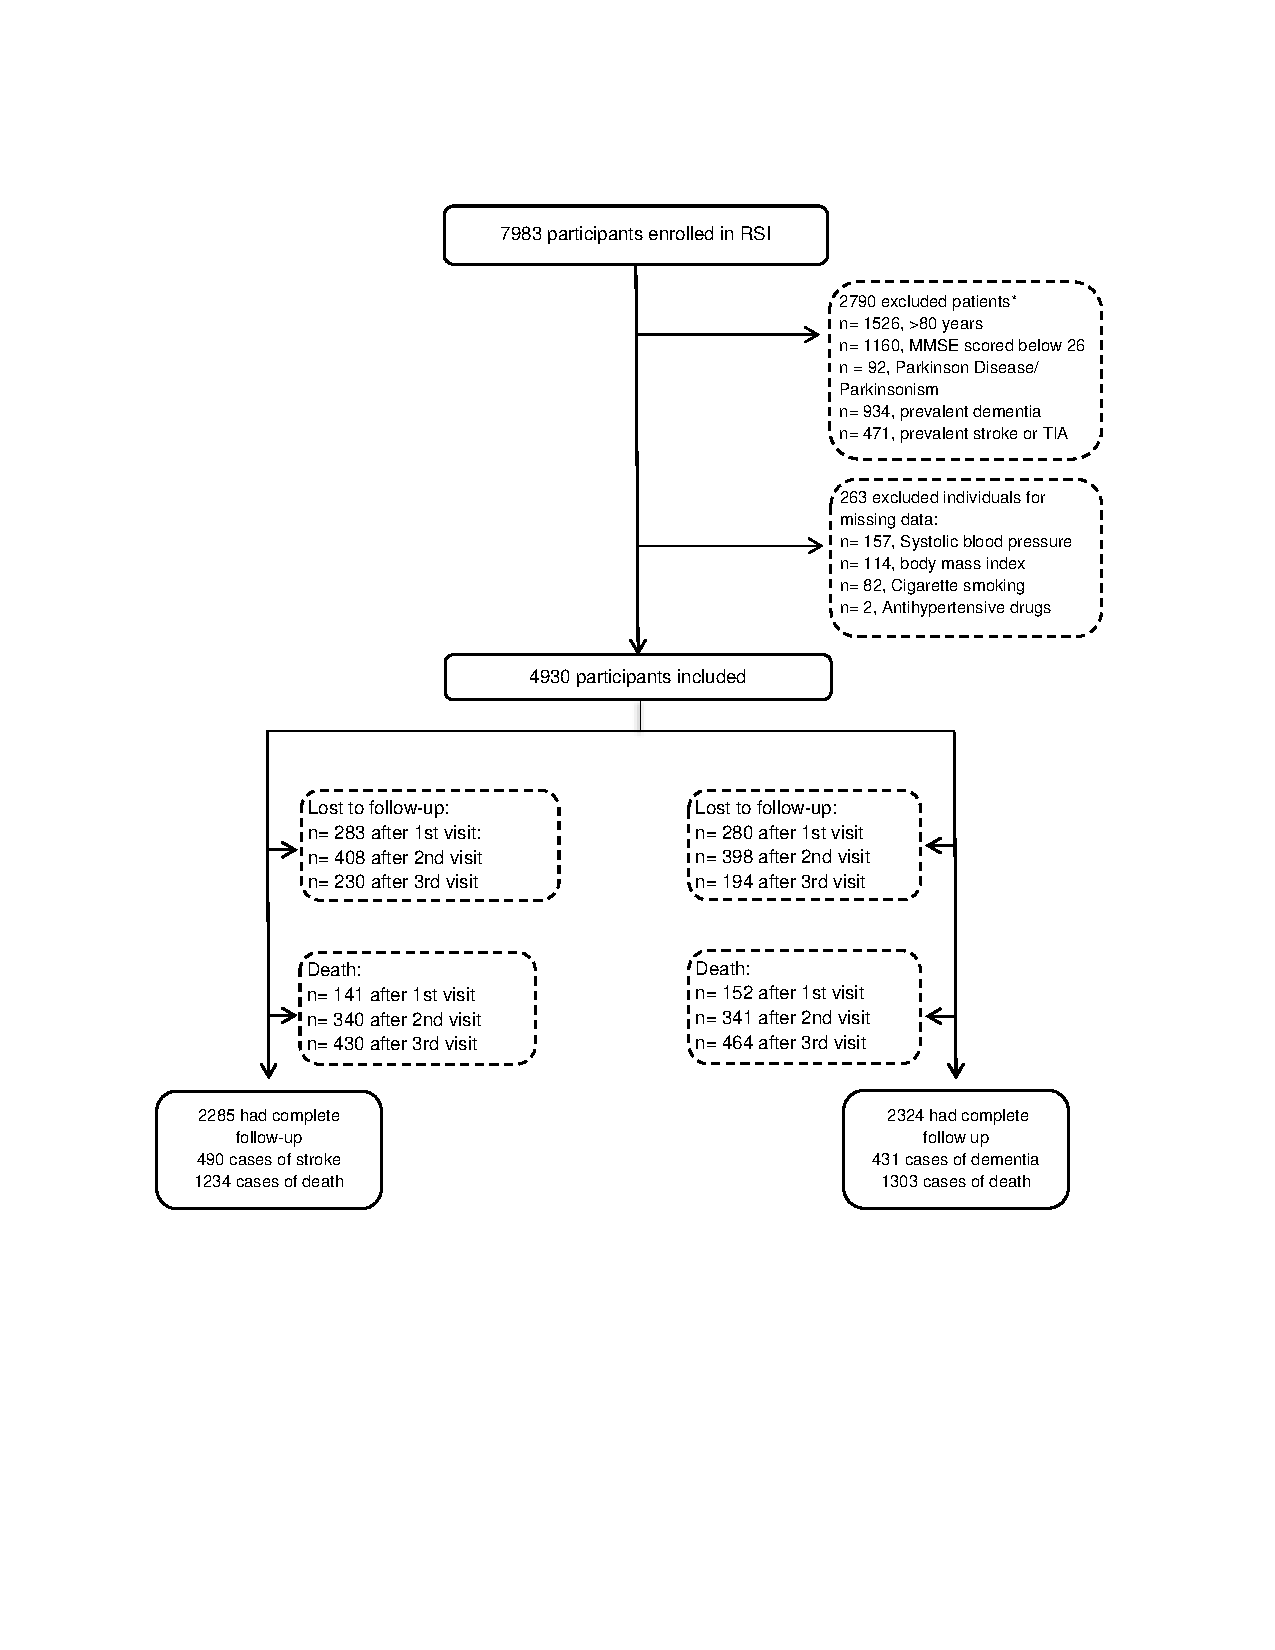
\includegraphics{figs/03_fig1.pdf}
\caption{(\#fig:03\_fig1)\textbf{Flowchart}. After a baseline block without stimulation, participants performed the attentional blink task during 20 minutes of anodal.}
\end{figure}



\hypertarget{statistical-analysis}{%
\subsection{Statistical Analysis:}\label{statistical-analysis}}

To estimate the risk of stroke and dementia under the described hypothetical interventions, we used the parametric g-formula, an extension of standardization to time-varying exposures and confounders. Under the assumptions of no unmeasured confounding and no model misspecification, this method provides an estimate of the risk of outcomes under full adherence to different hypothetical sustained interventions \autocite{taubman2009,garcia_aymerich2014,danaei_epid2013,vangenlonne2018,dickerman2019}.

The simplified steps for the parametric g-formula, using stroke as the outcome are described as follows:

\begin{enumerate}
\def\labelenumi{\arabic{enumi}.}
\item
  Fit parametric regression models for each of the time-varying covariates, as a function of baseline covariates and covariates history among participants followed up to time \emph{k}.
\item
  Fit parametric regression models for stroke and death, as a function of baseline covariates and covariates history among participants followed up to the time \emph{k}, using pooled logistic regression to approximate time-to-failure risk.
\item
  Use a Monte Carlo simulation to generate life histories for a pseudo-population of 10000 simulated individuals.
\end{enumerate}

\begin{enumerate}
\def\labelenumi{\alph{enumi}.}
\item
  Baseline covariates are randomly sampled with replacement from the original population.
\item
  The values of time-varying covariates are drawn from the parametric distribution in Step 1.
\item
  The value of the covariates that will be ``intervened'' on is set according to the defined strategy (skip this step for the ``natural course strategy'').
\item
  The predicted risk of dementia and death is calculated for each individual in the pseudo-population.
\end{enumerate}

\begin{enumerate}
\def\labelenumi{\arabic{enumi}.}
\setcounter{enumi}{3}
\item
  Calculate the mean predicted risk of stroke and death at 15 years in the pseudo-population.
\item
  Calculate the risk difference between each strategy and the natural course.
\item
  Repeat previous steps in 500 bootstraps samples to obtain the 95\% confidence interval (CI).
\item
  For each strategy repeat step 3 to 6.
\end{enumerate}

The same steps were performed with dementia as an outcome. Our primary analyses consisted of models with baseline confounders which included: age with a quadratic term, sex, APOE-ε4 carrier, history of type-II diabetes mellitus, history of heart disease, education level, baseline SBP with a cubic term. Additionally, we also included time-varying covariates: the visit process, SBP, cholesterol, BMI, alcohol intake, smoking status, hypertensive medications, incident heart disease, incident diabetes, incident cancer, incident transient ischemic attack and incident Parkinson Disease or Parkinsonism. Details on measurements of these variables are available in the online supplementary material (Measurements). When stroke was the principal outcome, we included dementia as a time-varying confounder, and vice versa. All covariates that were measured during the visit process were modeled under the condition of having attended the visit (Online resource, Table e-3). To probe for potential model misspecification, we estimated the difference between the observed mean value and the predicted mean value for each covariate (Online resource, Figure e-1, Figure e-2). We also conducted a sensitivity analysis of reordering the time-varying covariates to probe potential model misspecification.

The results are presented as the average causal effect under each hypothetical intervention at 15 years of follow-up compared to the natural course as a risk ratio and risk difference. For each intervention, we further report the cumulative proportion of participants who would have had to have been intervened on during the follow-up, to adhere to the strategy. We additionally presented the standardized cumulative incidence curves, comparing the risk over time under the natural course and the joint treatment strategy.

\textbf{\emph{Competing risk analysis:}} During follow-up, individuals can die before developing stroke and dementia, and interventions may affect the risk of death in our main analysis. For this reason, we estimate the risk of stroke and dementia taking into account that individuals can also progress to death. This means that the effect on our main outcome is through all pathways between the interventions and the outcome, including those possibly mediated by this competing event. We additionally run the primary analysis considering death as a censoring event, however the interpretation in this setting emulates a counterfactual world in which death could be entirely prevented, which would not be realistic and relies on additional stronger no-unmeasured-confounding assumptions \autocite{young2020}. Finally, we performed analysis considering the effect of each intervention in the composite outcome with death (i.e., stroke and death, dementia and death).

\textbf{\emph{Subgroup analysis:}} We repeated our primary analyses within the following subgroups: age 55 to 65 years; age between 66 and 80 years; women, men; without hypertensive medication at baseline; and free of heart disease at baseline.

All g-formula analyses were conducted using SAS 9.4 software and the GFORMULA macro that is publicly available at \url{http://www.hsph.harvard.edu/causal/software}. The SAS code for the GFORMULA macro call for our primary analysis is available on the following repository
\url{https://github.com/palolili23/ht_trial_gformula}.

\hypertarget{results-1}{%
\section{Results}\label{results-1}}

Table 1 shows the baseline characteristics of the study participants. The mean age of the participants was 66 years and 57\% were women. The mean SBP at baseline was 137 mmHg, and 24\% were current cigarette smokers.

\textbf{\emph{Stroke risk:}} During the 15 years of follow-up, there were 490 cases of incident stroke and 1234 deaths. The observed 15 years risk for stroke was 10.3\% and under the simulated natural course was 10.3\% (95\%CI: 9.3, 11.5). The risk of stroke under the different hypothetical treatment strategies are presented in Table 2. Overall, all interventions that lowered SBP under a threshold reduced the risk of stroke by approximately 10\% compared to the natural course during the study period. Although all interventions on SBP had a similar association with risk of stroke, the most intensive treatment strategy studied (``maintaining SBP below 120 mmHg'') required intervening in 98\% of the population at some point in follow-up, which involved 15\% more people compared to all other strategies. By contrast, smoking cessation was associated with a reduction in stroke risk by 7\% (RR 95\%CI: 0.89, 0.97) compared to the natural course, and required an intervention on only 26\% of the population. All joint interventions showed a larger reduction in the risk of stroke. For example, lowering SBP by 20\% if above 140 mmHg and quitting smoking was associated with a 17\% (RR 95\% CI: 0.71, 0.94) reduction in the risk of stroke over the study period compared to the natural course as observed in Figure 2A.

\textbf{\emph{Dementia risk:}} During the 15 years of follow-up, there were 431 cases of dementia and 1303 deaths. The observed 15-year risk for dementia was 8.9\% and under the simulated natural course was 9.2\% (95\% CI: 8.2, 10.3\%). The risk of dementia under the different hypothetical interventions are shown in Table 3. Overall, none of the treatment strategies involving SBP were associated with substantial changes in risk of dementia. For example, the treatment strategy ``maintaining SBP below 120 mmHg'' was associated with a 6\% (RR 95\% CI: 0.90, 1.24) increase in dementia risk compared to the natural course. This pattern was likewise seen for the treatment strategy of smoking cessation and joint treatment strategies involving lowering SBP and smoking cessation. For example, lowering SBP by 20\% if above 140 mmHg and quit smoking was associated with an increment in dementia risk of 5\% (RR 95\% CI: 0.92, 1.20) as observed in Figure 3A.

Alternative analyses for competing event: Given that death was modeled as a competing event for both outcomes (stroke and dementia), we present the effect of the intervention ``lowering 20\% of SBP if above 140 mmHg and quit smoking'' on the risk of death in Figure 2B and Figure 3B respectively. Treating death as a censoring event and as part of a composite outcome did not meaningfully change the results, as presented in the online resource, Table e-4, e-5, e-11, e-12.

\textbf{\emph{Subgroup analyses:}} Table 4 provides estimates for the treatment strategy ``lowering 20\% of SBP if above 140 mmHg and quit smoking'' on the risk of stroke and dementia by subgroups (age, sex, without hypertension medication at baseline, free of heart disease at baseline) compared to the natural course. Estimates were relatively consistent for stroke risk across subgroups, with the exception of individuals with age below 65 years among whom there appeared to be a much stronger association (RR: 0.75, 95\% CI: 0.56, 0.98).For dementia risk, subgroup analyses present similar findings. Additional treatment strategies are presented in the online resource, Table e-6 to e- 11, e-14 to e-19.

\hypertarget{discussion-1}{%
\section{Discussion}\label{discussion-1}}

Our study suggests that intervening on blood pressure could reduce stroke risk by approximately 10\% over 15 years of follow-up in a population-based setting, and that combining such interventions with smoking cessation could result in an overall reduction of 18\%. In contrast, our study is consistent with these same interventions having null or opposite effects on risk of dementia, taking into account that these estimates could be affected by how the interventions may decrease the risk of death.

Our results on stroke risk are comparable in direction but not quite in magnitude of prior studies' effect estimates. A previous meta-analysis of randomized trials has shown that a 10 mmHg reduction in blood pressure decreases the risk of stroke by 27\%, though this effect was observed in a high-risk population of individuals with cardiovascular diseases \autocite{ettehad2016}. The most comparable observational study to ours was one emulating hypothetical treatment strategies to reduce SBP in middle-aged (i.e., baseline mean age 46.1 years or about 20 years younger that our study) healthy individuals from Norway, also using the g-formula. This study showed that a 23 mmHg average reduction in blood pressure of 120 mmHg and above resulted in a 45\% reduction in stroke risk over a 15 year period \autocite{vangenlonne2018}. The difference in the risk estimates might be due to differences in the average age of the study populations. Of note, no differences in proportional risk reductions were reported in trials involving persons with systolic blood pressure \textless130 mmHg and those at high risk (≥160 mmHg) \autocite{ettehad2016}. Our study also adds to these prior studies by considering a joint intervention with smoking cessation, although our combined strategies appears to reduce stroke risk by a much lower amount (18\%) than those reported previously in observational studies (35-55\%) {[}8--10{]}.

To compare the results from our hypothetical intervention on blood pressure (dropping below 120 or 140 mmHg over time) in dementia risk with previous research, we must consider the differences in the eligibility criteria, treatment strategies and analytical choices. Our target trial by design follows similar treatment strategies such as the Systolic Blood Pressure Intervention Trial (SPRINT) MIND trial, however this trial considered eligible individuals as those who had risk of cardiovascular disease \autocite{williamson2019}, which represents a small subgroup of our population-based cohort. (Specifically, at most 290 individuals in the Rotterdam Study would meet criteria at baseline, based on our assessments of SBP, presence of cardiovascular disease other than stroke and history of diabetes.) Similarly, since previous trials were primarily designed to assess the effect of antihypertensive medication on the risk of stroke and did not have dementia as their primary outcome, they were tailored to a specific subgroup of individuals who required treatment. Eligibility criteria in other trials included having had a history of stroke, being above 80 years old and having a SBP above 160 mmHg \autocite{ace_inhibitors2000,prince1996,forette2002,progress2003,lithell2003,diener2008,anderson2011,williamson2019,bosch2019}. Furthermore, assessing the comparability of our findings with prior observational studies requires caution. A recent meta-analysis by Ding et al.~have studied the effect of taking any antihypertensive medication and specific antihypertensive medications and the risk of dementia stratified by SBP including five large population-based cohort \autocite{ding2020}. However, they assess the effect being on treatment at baseline and only include baseline covariates for adjustment. Similarly, Want et al.~stratify individuals by longitudinal blood pressure patterns (mid-life and late-life normotension/hypertension), but covariates are measured during two of the six visits \autocite{walker2019}. In contrast, we assessed the sustained effect of lowering SBP over time given time-updated covariates. Last, we consider that our findings reflect the relevance of the competing event of death by other causes, and how estimates are likely affected by the effect of interventions on the risk of death, and give a more comprehensive view of the implications of these results. This will be especially important when we stratify by characteristics that have a different survival distribution, as we observe in the different direction of the effects among women vs.~men \autocite{beam2018}. Reconsidering these points as part of how we frame research question and analytical decisions when using observational data, will have a direct impact on results interpretation and clinical translation.

By leveraging a rich dataset in a population-based observational study, high-quality and frequent assessments of outcomes and key covariates, and the use of the parametric g-formula to account for the complex confounding structure assumed, we emulated a ``target trial'' that may be of key public health interest but would not be easily conducted as a randomized trial. However, like any observational data analysis, several assumptions need to be carefully weighed. The possibility of unmeasured confounding remains, and in particular we were unable to adjust for covariates such as types of antihypertension medications, LDL (as separate from total cholesterol), glucose and frailty in our analysis. Likewise, we used MMSE as a screening tool and excluded individuals with Parkinson disease or parkinsonism symptoms at baseline, but it is possible that persons with subclinical cognitive impairment might be included in our analysis at baseline or during follow-up \autocite{joe2019}. Self-reported smoking status is also subject to measurement error, although we did assess the consistency of our measurements over time. In addition, the parametric g-formula relies on several strong modeling assumptions. As reported in the online resource Figure e-1, Figure e-2, we observed an agreement between the mean estimated values of each variable (outcomes and covariates) under the natural course with their observed values, which supports but does not prove these model specifications hold \autocite{taubman2009}. Furthermore, we did not assess the effect of the hypothetical interventions in the specific clinical phenotypes of each disease, since numbers on the disaggregated clinical subtypes are small and is further complicated by each subtype being a competing event for each other. However, the effect of lowering blood pressure may effect in the risk of each clinical subtype in different magnitude and should be addressed in future studies.

Finally, another key point to reflect upon in interpreting our specified treatment strategies is that we did not, in fact, specify how SBP would be lowered. This means our estimates are based on the consistency assumption that lowering SBP through any available means (e.g., dietary changes, medication use, other lifestyle changes) would have the same effect on stroke or dementia risk, or otherwise are at best interpretable as estimates for an effect of a weighted average of several SBP-lowering strategies with weights determined by the frequency that the particular strategies occur in our specific population \autocite{waterkills,hernan2011}. Future studies that have more detailed assessments of these various SBP-lowering treatments are needed to disentangle treatment variation relevance and build upon this initial study. Furthermore, smoking cessation is one of several more specific behavioral interventions that could be assessed, as well as other metabolic factors described in current guidelines\autocite{johnson2019,lancet2020}. Implementing the target-trial framework and defining research questions to study more refined or further specified treatment strategies is a crucial next step. Doing so will require rich, longitudinal data on the specific interventions under study; the level of specificity in the research questions that can be studied is hampered in part by the data currently available. Thus, while there are certainly limitations in terms of ambiguity to the interventions studied in the current paper, they represent an improvement (in terms of clarity and for informing decision-making) over etiologic studies that address SBP's effects with a simplified version of the complexity of real data, and a step toward the types of interventions we may consider in practice.

Given previous considerations, studying population-level interventions as done here is particularly suitable for public health research, in that we can better understand how particular recommendations may affect stroke or dementia risk at the population-level rather than as estimated in high-risk subpopulations. Importantly, while the possible effect of blood pressure control on dementia risk remains debated, our findings nonetheless align with the recent WHO Report's recommendation that lowering blood pressure has substantial benefits (in terms of stroke risk and mortality, here) that may motivate blood pressure control regardless of its possible effects on dementia risk\autocite{who_dementia2019}.

\hypertarget{references-1}{%
\section{References}\label{references-1}}

\hypertarget{chapter4}{%
\chapter{Towards a clearer causal question underlying the association between cancer and dementia}\label{chapter4}}

\chaptermark{Pin 1 and risk of dementia}

\newpage

\hypertarget{abstract-2}{%
\section{Abstract}\label{abstract-2}}

\textbf{Background:} Several observational studies have described an inverse association between cancer diagnosis and dementia. Several biological mechanisms and sources of bias have been proposed. Since bias cannot be assessed without a clear causal question, we propose to study the controlled direct effect of the protein Pin1 on the risk of dementia. With this case-study, we will outline the needed assumptions and potential sources of bias and exemplify how these translate into the analytic decisions under the guidance of causal directed acyclic graphs

\textbf{Methods:} We used data from the Rotterdam Study, a population-based cohort. We estimate the association between cancer diagnosis (as proxy for Pin1) and dementia diagnosis using two different proxy methods and with confounding and censoring for death addressed with inverse probability weights. We estimate and compare the complements of a weighted Kaplan-Meier survival estimator at 20-years of follow-up.

\textbf{Results:} Out of 3634 participants, 899 (25\%) were diagnosed with cancer, of whom 53 (6\%) had dementia, and 567 (63\%) died. Among those without cancer, 15\% (411) were diagnosed with dementia, and 667 (24\%) died over follow-up. Depending on the confounding and selection bias control, and the way in which cancer was used as a time-varying proxy, the risk ratio ranged from 0.70 (95\%CI: 0.49, 0.93) to 1.05 (0.79, 1.29).

\textbf{Conclusion:} Being explicit about the underlying mechanism of interest and defining a clear causal contrast is key to maximize what we can learn about this association given available or readily-collected data, and to defining, detecting, and preventing potential biases.

\newpage

\hypertarget{towards-a-clearer-causal-question-underlying-the-association-between-cancer-and-dementia}{%
\section{Towards a clearer causal question underlying the association between cancer and dementia}\label{towards-a-clearer-causal-question-underlying-the-association-between-cancer-and-dementia}}

Many observational studies have consistently found that individuals with cancer have a lower risk of developing dementia when compared to individuals with no history of cancer \autocite{ma2014,hanson2016,vanderwillik2018,ospina2020}. These findings have motivated substantial research toward mechanistic explanations, including molecular and genetic pathways that may explain this association\autocite{behrens2009,harris2014,nudelman2019,Papin2020,driverbiogeront2014,olson2019,li2021,driverpin2015}. These research questions have led to discussions of repurposing or augmenting current cancer treatments, including chemotherapy, for dementia\autocite{snyder2017}.

Nevertheless, inferring any treatment or mechanistic effects from the observed cancer-dementia inverse association is not straightforward. Researchers have raised concerns related to the competing event of death, unmeasured confounding, and ascertainment error that could explain these results\autocite{driverbiogeront2014,ganguli2015}. However, understanding these or other sources of bias first requires making explicit a causal question. Moreover, enumerating an explicit causal question is one step toward tying a research study to a question that is relevant to decision-making\autocite{didelez2016,labrecque2017}.

To illustrate the complexities of inferring hypothetical or available cancer treatments' effects on dementia from the observed cancer-dementia association, we focus on a specific question conceptualizing the Pin1 enzyme as the target of intervention. Previous animal studies have shown that Pin1 enzyme over-expression promotes tumorigenesis, while its down-regulation is attributed to mechanisms that contribute to neurodegeneration and amyloid deposition\autocite{driverpin2015,angelucci2017,li2021}. If we -- hypothetically speaking -- one day could develop a drug that increases Pin1 expression specifically in brain tissue in hopes of preventing dementia, we could pose the question as: \emph{What is the effect of this Pin1-targeting drug on the risk of dementia over time compared to standard treatments?}

To explore how we might learn about this effect using real-world data on cancer and dementia, we progressively build a causal directed acyclic graph (DAG) to connect this question to the observable data and the assumptions we rely on to study the effect. We exemplify these challenges and how they translate into the analytic decisions using data collected from the Rotterdam Study, a population-based cohort study. In our discussion, we describe how other investigators may expand this exercise for other possible causal questions, including repurposing existing chemotherapy regimens or identifying other novel drug targets.

\hypertarget{methods-2}{%
\section{Methods}\label{methods-2}}

\hypertarget{overview-of-the-causal-structure}{%
\subsection{Overview of the causal structure}\label{overview-of-the-causal-structure}}

If this hypothetical Pin1-targeting drug was developed, the best way to understand its effect on dementia risk would be to have a well-conducted randomized trial in which we randomize eligible participants in late midlife (e.g., ages 50-60 years) to receive this drug or not, and closely monitor dementia diagnosis over a lengthy follow-up. Since this drug is not currently available, at best we can use observational data on Pin1 expression measurements. For example, suppose that a biomarker test was available to measure Pin1 and we measured this biomarker in stored baseline blood samples from late-midlife participants recruited for a population based-cohort.

In the observational setting, confounding could explain the observed association between Pin1 and dementia. In the causal diagram\autocite{whatif2020} in Figure 1, we present Pin1 expression as \(P_{t}\) and dementia diagnosis by time \(t+k\) as \(Y_{t+k}\). Both may share causes \(L_1\), and to assess the causal relationship between \(P_{t}\) and \(Y_{t+k}\) we would thus adjust for \(L_1\). Previous dementia studies have described age, sex, educational level and race/ethnicity as a minimal adjusting set of covariates\autocite{ospina2020}. However, environmental and behavioral factors such as smoking may translate into Pin1 over-expression\autocite{tan2010} and are also related to the development of dementia\autocite{dementia_lancet} and should therefore be adjusted for. Although \(L_1\) can be time-varying in nature, we only depict \(L_1\) at one time-point for readability.

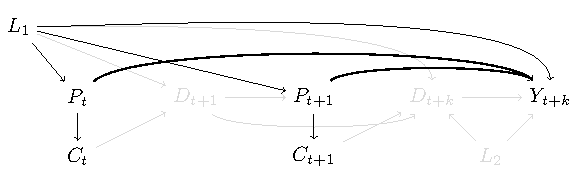
\includegraphics{04-cancer_files/figure-latex/unnamed-chunk-1-1.pdf}
\textbf{Figure 1. Causal directed acyclic graph highlighting confounding of the potential effect of Pin1 on risk of dementia.} Pin1 at time \(t\) is represented as \(P_t\); dementia at time \(t+k\) is represented as \(Y_{t+k}\); \(L_1\) represents shared causes of Pin1 and dementia, such as smoking. To isolate the effect of \(P_t\) on \(Y_{t+k}\) we need to block the backdoor path \(Y_{t+k} \leftarrow L_1 \rightarrow P_t\). Gray nodes and arrows are described progressively in Figures 1-5.

Currently, Pin1 expression is not an available biomarker for population-based research, so at best we can only rely on a proxy for it. Because Pin1 over-expression is present in tumors, and tumors are only diagnosed through biopsies, previous studies have speculated that Pin1 over-expression partly explains the inverse association between cancer diagnosis and dementia, though Pin1 was not explicitly part of the research question\autocite{driver2012,musicco2013,freedman2016,bowles2017,frain2017,schmidt2017,sun2020,ording2020}. Unlike measuring Pin1 at the same time for all participants (though this would not necessarily mean this would be the ideal time to measure it, we discuss this point further in the discussion section), cancer diagnosis is collected during follow-up. We depict this feature in Figure 2, where \(C_t\) and \(C_{t+1}\) represent \emph{cancer diagnosis} over time, the measured proxy of \(P_{t}\) and \(P_{t+1}\) respectively. Although this means we would measure the association between cancer diagnosis over time and dementia in the observed data, we are assuming that the captured effect is only through the pathway that involves Pin1 expression over time. That is, we only have measurements of \(C_{t+1}\) and \(Y_{t+k}\) and some subset of \(L_1\), but our question remains focused on the effect of \(P_t\).

We note that this means we already are changing our question from one of estimating the effect of Pin1 to one that is testing the sharp causal null hypothesis that Pin1 has no effect on dementia in any individuals. That is, an association between cancer and dementia is at best evidence against a null effect, and it would take substantial and unknown assumptions about the relationship between Pin1 and cancer diagnosis to describe how the magnitude of a cancer-dementia association is related to the likely magnitude of a Pin1-dementia effect.

\begin{figure}
\centering
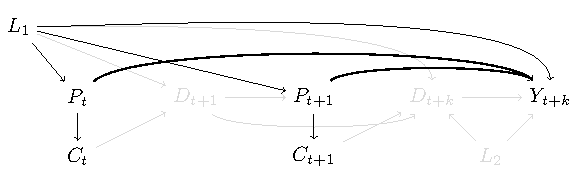
\includegraphics{04-cancer_files/figure-latex/unnamed-chunk-2-1.pdf}
\caption{\label{fig:unnamed-chunk-2}Figure 2.}
\end{figure}

\textbf{Figure 2. Causal directed acyclic graph highlighting the use of incident cancer diagnosis as a proxy for Pin1 expression.} Pin1 at time \(t\) and \(t+1\) are represented as \(P_t\) and \(P_{t+1}\), respectively; dementia at time \(t+k\) is represented as \(Y_{t+k}\); \(L_1\) represents shared causes of Pin1 and dementia; incident cancer diagnosis at time \(t\) and \(t+1\) are represented as \(C_t\) and \(C_{t+1}\). To isolate the effect of \(P_t\) and \(P_{t+1}\) on \(Y_{t+k}\) we need to block the backdoor path \(Y_{t+k} \leftarrow L_1 \rightarrow P_t\) and \(Y_{t+k} \leftarrow L_1 \rightarrow P_{t+1}\). Although we represent \(L_1\) as a single node for readability, \(L_1\) is time-varying too. Gray nodes and arrows are described progressively in Figures 1-5.

Another challenge that arises when choosing cancer diagnosis as the proxy for Pin1 is defining the time zero, i.e.~the time when eligibility criteria are met, ``treatment'' is assigned, and screening for dementia would begin\autocite{hernan2016}.Emulating the eligibility criteria to participate in a trial for Pin1-targeting drugs will not necessarily be possible in a cohort setting recruiting participants for discordant reasons. Moreover, the latter may not align with the moment at which cancer diagnosis is measured since it happens continuously over follow-up and this situation may introduce immortal-time bias\autocite{hernan2016}. For example, a study performed using data from the Framingham Heart Study\autocite{driver2012} defined the exposed group with cancer as those participants with prevalent or incident cancer diagnosis (alternatively defined as ``ever cancer''\autocite{hanson2016}). This meant that a participant who had cancer diagnosis over follow-up contributed all their person-time to the cancer arm, including the time prior to the cancer diagnosis. By defining the exposure after the time of inclusion to the cohort, only participants who remain alive and free of dementia diagnosis over follow-up can be defined as ``ever cancer''\autocite[\textcite{hernan2016}]{anderson1983}.

This problem is partly mitigated by recognizing the time-varying nature of cancer diagnosis. Some studies have considered cancer diagnosis as a time-dependent exposure\autocite{white2013,hanson2016,bowles2017}. The price we pay for this approximation is that implicitly, this means that Pin1 would over-express at the time of cancer diagnosis and not before, which is biologically implausible. The time between first biological changes that eventually can lead to cancer and cancer manifestation can range between five and forty years\autocite{nadler2013}. Moreover, cancer diagnosis will only be measured in the subset of participants who are alive over follow-up. Thus, in Figure 3 we included death prior to cancer diagnosis as \(D_{t+1}\) and an arrow between \(D_{t+1}\) and \(P_{t+1}\) that represents a deterministic association such as that \(P_{t+1}\) is only observed if \(D_{t+1}\) is zero. In addition, we added an arrow between \(L_1\) and \(D_{t+1}\), since covariates such as smoking may affect Pin1 over-expression but also affect the risk of death due to other causes such as from chronic obstructive pulmonary disease.

\begin{figure}
\centering
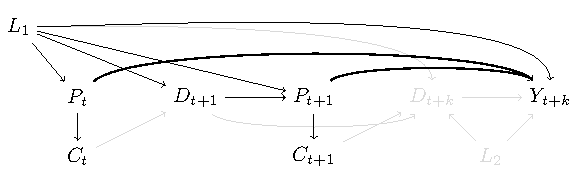
\includegraphics{04-cancer_files/figure-latex/unnamed-chunk-3-1.pdf}
\caption{\label{fig:unnamed-chunk-3}Figure 3.}
\end{figure}

\textbf{Figure 3. Causal directed acyclic graph highlighting the time-varying nature of cancer diagnosis and immortal time bias.} Pin1 at time \(t\) and \(t+1\) are represented as \(P_t\) and \(P_{t+1}\), respectively; dementia at time \(t+k\) is represented as \(Y_{t+k}\); \(L_1\) represents shared causes of Pin1 and dementia; incident cancer diagnosis at time \(t\) and \(t+1\) are represented as \(C_t\) and \(C_{t+1}\). \(D_{t+1}\) represents death at time \(t+1\), cancer diagnosis at \(t+1\) can only be measured among those who are alive at \(t+1\). Gray nodes and arrows are described progressively in Figures 1-5.

Another challenge to address is related to death as a competing event for dementia, represented in Figure 4. For interpretability we exclude the time-varying process of cancer diagnosis and focus on Pin1 (and cancer diagnosis) as it had been measured in all participants at time \(t+1\). Given that some participants may die prior to dementia diagnosis, we can only measure dementia over follow-up in the individuals who survive long enough to have a dementia diagnosis. In the causal diagram of Figure 4 we include a node for death after the exposure \(C_{t+1}\) has been measured, represented as \(D_{t+k}\) and which acts as a competing event of \(Y_{t+k}\) because if a participant dies by \(t + k\), the participant cannot subsequently develop dementia. Furthermore, since \(D_{t+k}\) and \(Y_{t+k}\) are events related to aging and its consequences, \(L_2\) represents the shared causes of both events such as cardiovascular conditions. We also include an arrow between \(L_1\) and \(D_{t+1}\) following the argument discussed previously.

\begin{figure}
\centering
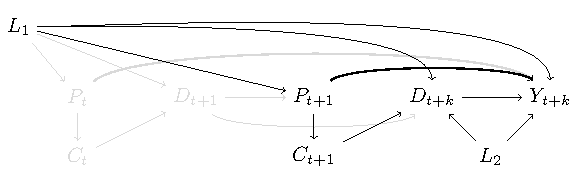
\includegraphics{04-cancer_files/figure-latex/unnamed-chunk-4-1.pdf}
\caption{\label{fig:unnamed-chunk-4}Figure 4.}
\end{figure}

\textbf{Figure 4. Causal directed acyclic graph highlighting death as a competing event of dementia} Pin1 at time \(t\) and \(t+1\) are represented as \(P_t\) and \(P_{t+1}\), respectively; dementia at time \(t+k\) is represented as \(Y_{t+k}\); \(L_1\) represents shared causes of Pin1 and dementia; incident cancer diagnosis at time \(t\) and \(t+1\) are represented as \(C_t\) and \(C_{t+1}\); \(D_{t+1}\) represents death at time \(t+1\). In this graph we only focus attention to the exposure as if it was measured for all at time \(P_{t+1}\). We include \(D_{t+k}\) as death at time \(t+k\) since \(Y_{t+1}\) is only observable when participants are alive at \(t+k\). \(L_2\) represents possible shared causes of dementia and death (such as cardiovascular comorbidities). Pin1 may affect the risk of death through cancer diagnosis, represented as an arrow between \(C_{t+1}\) and \(D_{t+k}\). To isolate the direct effect of \(P_{t+1}\) and \(Y_{t+k}\), we have to block the backdoor pathway from \(Y_{t+k} \leftarrow L_2 \rightarrow D_{t+k} \leftarrow C_{t+1} \leftarrow P_{t+1}\) and \(Y_{t+k} \leftarrow D_{t+k} \leftarrow L_1 \rightarrow P_{t+1}\). Gray nodes and arrows are described progressively in Figures 1-5.

In the setting where \(P_{t+1}\) represented the targeted-drug for Pin1, and if this drug had no systemic beneficial or harmful side-effects such as that there is no arrow between \(P_{t+1}\) and \(D_{t+k}\), a total effect would quantify the effect of \(P_{t+1}\) on \(Y_{t+k}\) that does not include any pathway mediated through \(D_{t+k}\)\autocite{young2020}. However, in the context of cancer diagnosis as the proxy for Pin1 over-expression, we cannot rule out the effect of cancer diagnosis on death, represented as the arrow between \(C_{t+1}\) and \(D_{t+k}\). In this setting, a total effect of \(P_{t+1}\) in \(Y_{t+k}\) includes the indirect causal pathway mediated by the effect of cancer diagnosis on mortality, which may translate into an inverse association\autocite{young2020}.

To isolate the direct effect of \(P_{t+1}\) in \(Y_{t+k}\) through measurement of \(C_{t+1}\) we have at least two alternatives of causal questions we can ask. One, we can imagine a causal question where we decompose the total effect of cancer by the different pathways that affect dementia and death separately\autocite{stensrud2020}. Two, we can define a scenario where death could have been prevented. The latter is defined as the controlled direct effect, where death is considered as an independent censoring event by relying on the assumption that we have measured all shared causes \(L_2\) to block the pathway \(Y_{t+k} \leftarrow L_2 \rightarrow D_{t+k} \leftarrow C_{t+1} \leftarrow P_{t+1}\). Previous studies have defined death as a censoring event \autocite{frain2017}, although failed to explicitly define the independent censoring assumption and did not consider its plausibility. Moreover, adjusting for time-fixed shared causes between dementia and death may be insufficient to block this pathway, and therefore time-varying measurements of \(L_2\) should be considered.

To summarize, the complexity of the causal structure that describes the effect of Pin1 on dementia risk while proxying Pin1 with cancer diagnosis illustrates the potential sources of bias, as observed in Figure 5. Even so, this is a simplified version since we omitted additional arrows from \(L_1\) to \(C_t\) and \(C_{t+2}\) for brevity, as well as other sources of measurement error and the time-varying nature of all nodes and feedback loops between them, which would further complicate interpretability\autocite{whatif2020}.

\begin{figure}
\centering
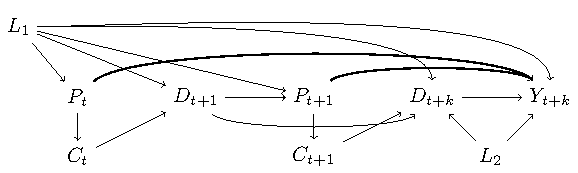
\includegraphics{04-cancer_files/figure-latex/unnamed-chunk-5-1.pdf}
\caption{\label{fig:unnamed-chunk-5}Figure 5.}
\end{figure}

\textbf{Figure 5. Causal directed acyclic graph depicting multiple challenges to using the proxy of cancer diagnosis to study the effect of Pin1 on risk of dementia.} Pin1 at time \(t\) and \(t+1\) are represented as \(P_t\) and \(P_{t+1}\), respectively; dementia at time \(t+k\) is represented as \(Y_{t+k}\); \(L_1\) represents shared causes of Pin1 and dementia; incident cancer diagnosis at time \(t\) and \(t+1\) are represented as \(C_t\) and \(C_{t+1}\); \(D_{t+1}\) and \(D_{t+k}\) represents death at time \(t+1\) and \(t+k\); \(L_2\) represents possible shared causes of dementia and death. The distinct challenges were highlighted separately in Figures 1-4.

We now turn to an application where we show how these challenges translate into analytic decisions. We will show ways to mitigate or better understand bias to the best of the available data's abilities in an attempt to inform the possible effect of Pin1 on dementia risk.

\hypertarget{the-rotterdam-study}{%
\subsection{The Rotterdam Study}\label{the-rotterdam-study}}

We use data collected in the Rotterdam Study, a population-based prospective cohort study among persons living in the Ommoord district in Rotterdam, the Netherlands. Recruitment and initial assessments were held between 1990 and 1993, a second wave of recruitment was held between 2000 and 2001. Participants from the first sub-cohort had follow-up visits between 1993-1995, 1997-1999, 2002-2005, and 2008-2010, while the second sub-cohort had follow-up visits between 2004 and 2005, and between 2011 and 2012\autocite{ikram2020}. All participants had data on history of cancer and dementia and incident diagnosis, collected from medical records of general practitioners (including hospital discharge letters) and through linkage with national registries. Date and cause of death was collected via municipal population registries. These ascertainment methods imply that the Rotterdam Study has functionally no loss to follow-up with respect to dementia diagnosis and death

Eligibility criteria included: ages 60 to 70 years at study entry; no history of cancer diagnosis, no history of dementia diagnosis; and free of cognitive decline (defined by a Mini Mental Score \textless26). Out of 10998 persons who participated at study entry, 3634 were considered eligible. Time to cancer diagnosis, time to dementia diagnosis and death status was measured for all participants. All participants were followed from study entry until dementia diagnosis, death or 20 years after their individual baseline date, whichever occurred first. Given that participants from the second sub-cohort were followed for 15 years, we assume that they would have had a similar distribution of dementia risk and mortality as the first subcohort, between year 15 and 20 of follow-up.

\hypertarget{statistical-methods}{%
\subsection{Statistical Methods}\label{statistical-methods}}

We illustrate the association between cancer and dementia diagnosis under two scenarios, the first of which replicates a common analytic strategy and the second which mitigates some (but not all) the biases described above. Scenario A replicates the setting that defines cancer proxy as \emph{``cancer ever vs.~never''}\autocite{driver2012}, meaning we compare dementia outcomes in individuals who ever develop cancer during follow-up to those who were not observed to develop cancer during follow-up. Scenario B defines cancer diagnosis as time-varying meaning that time prior to cancer diagnosis is allocated to the non-exposed arm, and the time after cancer diagnosis to the exposed arm. To address confounding, we fit inverse probability treatment weights, stabilized and truncated at the 99th percentile. In Scenario A, weights were defined as the inverse of the probability of cancer diagnosis conditional on baseline covariates such as age at study entry, sex, educational attainment, cohort, smoking status. In contrast, for Scenario B, weights were defined to represent the product of the inverse probability of being diagnosed with cancer over time, conditional on the time-varying covariate history prior to cancer diagnosis\autocite{hernan2000}. Baseline covariates included age at study entry, sex, ApoE4 status, educational attainment and the time-varying covariates such as smoking status, systolic blood pressure, body mass index and prevalent and incident hypertension and diabetes.

Inverse probability censoring weights for death were calculated, assuming independent censoring conditional on measured covariates. In Scenario A, weights represent the inverse of the probability of not dying conditional on cancer diagnosis (ever vs.~never) and baseline covariates such as age, educational attainment, ApoE4, and baseline measurements of smoking status, hypertension status, systolic blood pressure, BMI, history of diabetes and cohort. For individuals who died, their censoring weight is zero\autocite{whatif2020}. In Scenario B time-varying weights represent the product of the inverse probability of surviving in each year prior to \emph{t}, conditional on the measured shared causes of death and dementia. For an individual who has died by time \emph{t}, the year \emph{t} censoring weight is zero\autocite{young2020}. Weights were fitted including the same covariates used to estimate weights for time-varying cancer diagnosis, though we additionally added time-varying cancer, stroke, and heart disease diagnosis as predictors for death. Further details on modeling specifications and weights assessment are presented in the \textbf{eAppendix}.

To estimate the controlled direct effect of Pin1 on the risk of dementia, we compared the complement of a weighted Kaplan-Meier survival estimator for participants who developed cancer versus those who did not, with time indexed in years. The weights are time-varying by follow-up year, defined as a product of the year-specific inverse probability of treatment weights and the inverse probability of censoring by death weights. Estimates of the controlled direct effect are presented as 20-year risk differences (RD) and risk ratios (RR). All 95\% confidence intervals were calculated using percentile-based bootstrapping based on 500 bootstrap samples.

Estimates are presented as 20-year risk differences (RD) and risk ratios (RR). All 95\% confidence intervals were calculated using percentile-based bootstrapping based on 500 bootstrap samples. For illustrative and comparative purposes, we also calculated hazard ratios (HR). Hazards, unlike risks, inherently condition on surviving both dementia and death, and as such a causal interpretation is problematic\autocite{young2020}.

Since the conditional independent censoring assumption is untestable, we compute Peterson upper and lower bounds\autocite{peterson1976} to represent: (1) the extreme scenario of independence, that refers to a scenario were those who died would never develop dementia (lower bound) and (2) complete dependency, that refers to an scenario where those who died would have a dementia diagnosis prior to death (upper bound). The lower bound is calculated with the Aalen-Johansen estimator treating death as a competing event, and the upper bound is calculated with the Kaplan-Meier estimator for the combined outcome of dementia or death.

All analysis were performed using R. Code is provided in supplementary material and available in \url{https://github.com/palolili23/2021_cancer_dementia}.

\hypertarget{results-2}{%
\section{Results}\label{results-2}}

Participants had a mean age of 64.5 years, and 54\% (n=1979) were women (Table 1). Over follow-up, 25\% (n=899) developed cancer, with a median age of cancer diagnosis at 73 (IQR:69-78). From the total sample, 13\% (n=460) were diagnosed with dementia over follow-up with a median age of at 79 (IQR:75-83) years. Among participants with incident cancer, 6\% (n=53) had dementia diagnosis, 63\% (n=567) died over follow-up, and 31\% (n=279) remained alive and dementia-free at 20 years since study entry. In contrast, among participants free of cancer diagnosis over follow-up, 15\% (n=411) were diagnosed with dementia, 24\% (n=667) died over follow-up, and 61\% (n=1657) were alive and dementia-free at the end of follow-up. The proportion of participants in each possible status over follow-up and leading causes of death for both arms are presented as eFigure 1 and 2 in the eAppendix.

Results for all scenarios are presented in Table 2. Using Scenario A's analytic design and without adjusting for confounding or selection bias due to conditioning on death, we observe a protective association with a risk ratio (RR, 95\% Confidence interval) of 0.70 (0.49,0.93) and a hazard ratio {[}HR, (95\% Confidence interval){]} of 0.52 (0.39,0.69). Though adjusting for measured confounding only minimally changed the observed association, the association is closer to the null after including censoring weights for death {[}RR: 0.91 (0.65,1.19); HR: 0.72 (0.54,0.98){]}. In contrast, using Scenario B's analytic design, the fully adjusted model results in a RR of RR: 1.05 (0.79,1.29) and a HR of 1.09 (0.80,1.50), though confidence intervals cross the null. The cumulative incidence curves for dementia for participants free of cancer diagnosis and with incident cancer diagnosis, under Scenarios A and B, reflect that the difference between groups changes over time and flips direction when considering cancer as a time-varying proxy. Bounds (rather than point estimates) were wide and covered the null (Lower bound RR: 0.39; Upper bound RR: 2.08).

(ref:04\_fig6) \textbf{Figure 6. Risk of dementia under elimination of death over 20 years of follow-up by cancer diagnosis status.} Panel A. represents the scenario where cancer was considered as ``ever vs.~never''. Panel B. represents the scenario where cancer was considered as a time-varying proxy.

\textbackslash begin\{figure\}
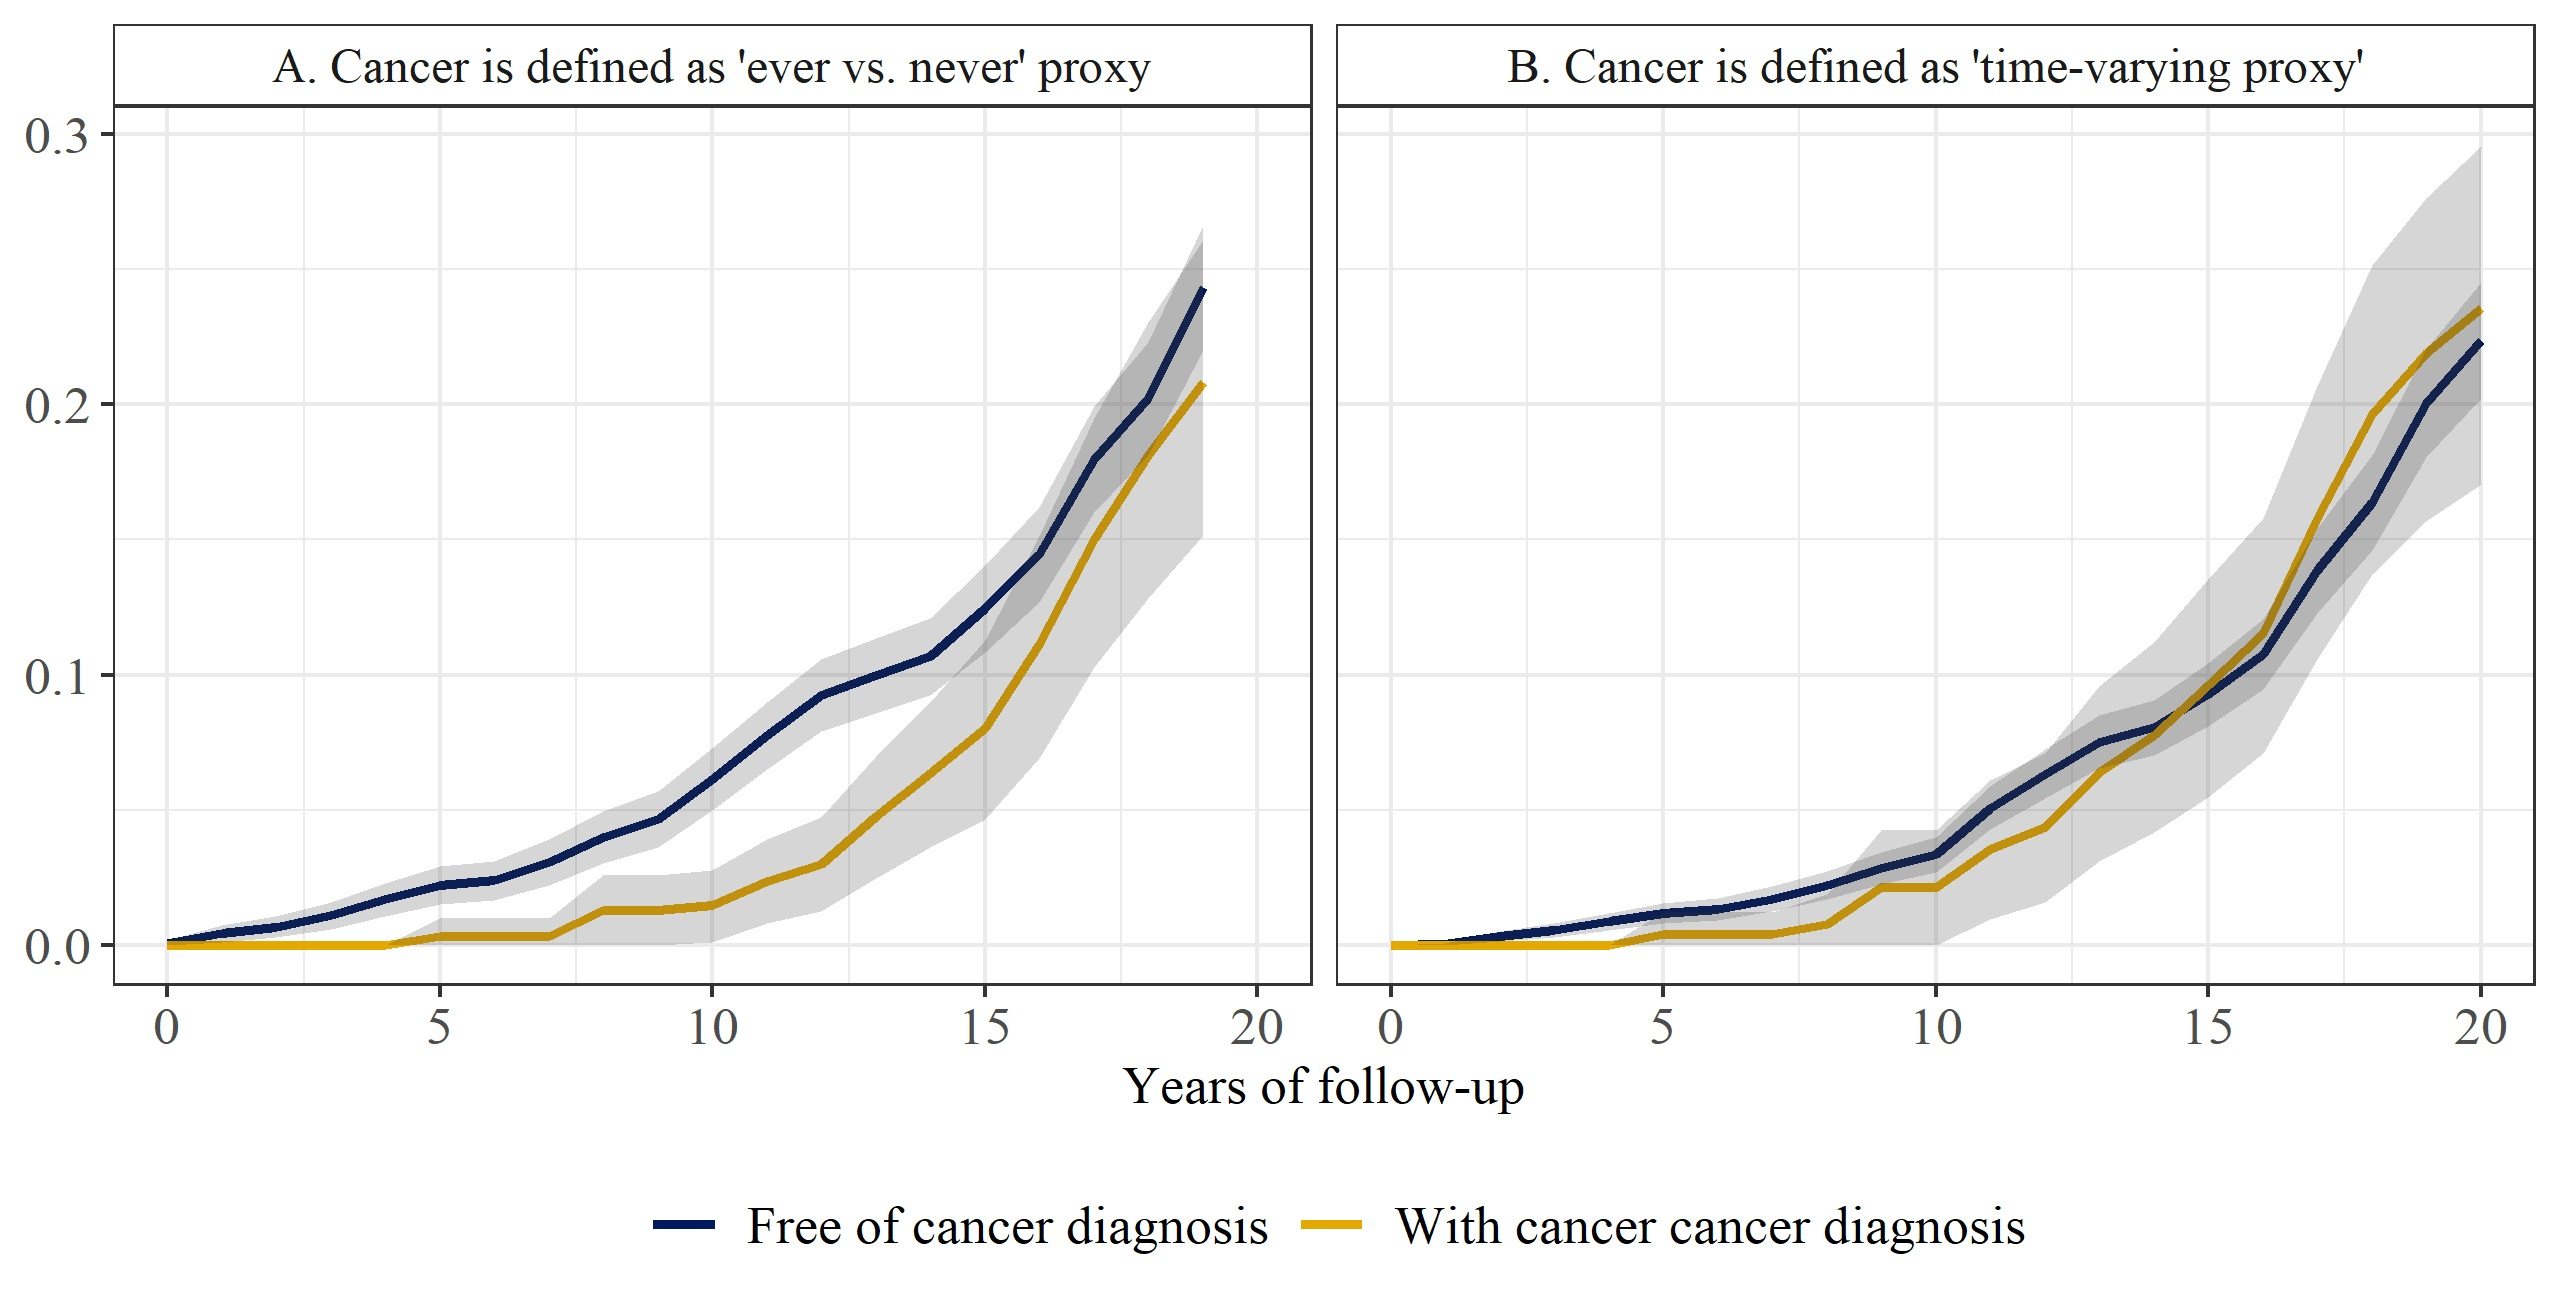
\includegraphics[width=35.56in]{V:/HomeDir/040609(Paloma Rojas)/My Documents/01_Projects/thesis_bookdown/figs/04_fig6} \textbackslash caption\{(ref:04\_fig6)\}\label{fig:unnamed-chunk-6}
\textbackslash end\{figure\}

\hypertarget{discussion-2}{%
\section{Discussion}\label{discussion-2}}

Several observational studies have defined ``cancer diagnosis'' as an exposure, although this does not represent a target for potential intervention or a modifiable risk factor. Instead, this variable is commonly used to represent a mechanism of interest that could not be measured. In this study we describe a particular research question of investigating a potential therapeutic drug-target of Pin1 expression, and discuss using cancer diagnosis as a proxy. By explicitly including Pin1 as part of the research question we connect the unmeasured mechanism of interest to the observed data outlining the data generation process. This practice helps to identify and disentangle potential sources of bias and can guide analytic decisions. We showed how estimates can change substantially according to alternative, yet explicit, assumptions.

For instance, a key challenge of cancer diagnosis as a proxy for Pin1 is the incapacity of defining a clear time zero\autocite{hernan2016}. In the setting where cancer diagnosis is defined as ``ever vs.~never'', this definition introduces immortal time bias. All results pertaining to this definition had an inverse association between cancer diagnosis and dementia, while results that did not introduce this particular form of immortal-time bias had point estimates closer to the null. Although we attempt to prevent this bias with statistical methods, we can only fully prevent it by having a clear definition of time-zero. Importantly, this definition does not depend on the collected data nor in analytic decisions: it relies on a deeper discussion related to when would be the best moment to potentially intervene on this biomarker and to what purpose. Thus, we hope that these unsolved questions guide future discussions and data collection efforts.

On the other hand, death as a competing event is a challenge that has some straightforward strategies, beginning first and foremost by choosing the causal parameter (or estimand) of interest\autocite[\textcite{rojas_medrxiv}]{young2020}. In this study we chose the controlled direct effect, which represents the effect of Pin1 (or cancer) in a setting where death due to cancer and other causes could have been prevented, yet without an explicit intervention, which makes it ambiguous. This is different than conceiving a drug-target that increases Pin1 expression only in brain tissue, with no side effects that could increase cancer risk (and thus, death due to cancer). As opposed to prior studies that implicitly address a direct effect, and that define censoring as ignorable\autocite{frain2017}, we show how point estimates change substantially when we include weights for death to relax the independent censoring assumption\autocite[\textcite{vangeloven2014}, \textcite{willems2018}, \textcite{young2020}]{weuve2012} when the estimand of interest is the controlled direct effect. Bounds to assess extreme scenarios of dependence between death and dementia\autocite{peterson1976} illustrate the wide range of possible point estimates that cross the null. This shows that even with the effort of adjusting for time-varying covariates, we may be far from meeting this assumption and thus better efforts to measure shared (time-varying) causes of dementia and death are needed. In addition, presenting the proportion of participants that died prior to dementia diagnosis in each arm, as well as the proportion of participants in each status over time, improves transparency and puts in evidence the limitations of the data to answer this question.

Pin1 is only one of the several mechanisms proposed by other investigators as an explanation for the inverse cancer-dementia relationship. Certainly, cancer diagnosis represents a complex and heterogeneous health condition that exceeds the representation of Pin1 expression. To understand how -- if at all -- the cancer-dementia association informs the potential effects of any other mechanism or treatment strategy, and its connection to collected data, we may require different causal representations. For example, if researchers used this association to inform the possible effects of different chemotherapeutics on cognitive decline among patients undergoing treatment for cancer, different challenges would arise for mapping the observed association to the hypothetical randomized trial underlying that new research question. Notably, that target trial, unlike the one considered here, would include cancer diagnosis as part of the eligibility, and thus researchers would need to instead grapple with how using data on persons without cancer is useful and useable\autocite{huitfeldt2016}.
Each question requires thinking about bias anew and each question brings its own set of challenges and opportunities.

We underscore that our study is just one case study for how observed associations between two diseases or health states may be disentangled to more transparently unveil possible mechanisms (and sources of bias) behind them, and how to maximize what we can learn about the potential mechanisms given available or readily-collected data. We hope to stimulate researchers first have a discussion about the exact research question, rather than trying to replicate the cancer and dementia relation in their dataset. Such discussion is needed to obtain meaningful conclusions.

\hypertarget{chapter5}{%
\chapter{How are we counting the dead in dementia studies?}\label{chapter5}}

Some \emph{significant} applications are demonstrated in this chapter.

\hypertarget{example-one}{%
\section{Example one}\label{example-one}}

\hypertarget{example-two}{%
\section{Example two}\label{example-two}}

\hypertarget{chapter6}{%
\chapter{Choosing questions before methods in dementia research with competing events and causal goals}\label{chapter6}}

Some \emph{significant} applications are demonstrated in this chapter.

\hypertarget{example-one-1}{%
\section{Example one}\label{example-one-1}}

\hypertarget{example-two-1}{%
\section{Example two}\label{example-two-1}}

\hypertarget{chapter7}{%
\chapter{Discussion}\label{chapter7}}

\chaptermark{Discussion}

\newpage

In this thesis, I aimed to study the effect of several potential targets of intervention related to dementia prevention that have had controversial results in previous observational studies, by applying causal inference theory and corresponding methods. In this section I will outline the principal findings of each project, laying the methodological challenges and the implemented solutions while reflecting on the broader implications of the research. Next, I will describe the potential future directions and briefly summarize the central points of this dissertation.

\hypertarget{principal-findings-and-broader-implications}{%
\section{Principal findings and broader implications}\label{principal-findings-and-broader-implications}}

The aim in \textbf{Chapter \ref{chapter2}} was to emulate a hypothetical randomized trial - a target trial - for estimating observational analogues to intention-to-treat and per-protocol effects of statins in the risk of dementia. In this study we found that individuals with sustained statin use, but not statin initiation alone, had reduced 10-year risks of dementia and dementia or death. Results should be interpreted with caution, due to the small number of statin initiators and number of dementia events, plus potential residual confounding. Nonetheless, these findings show how important it is to define and estimate per-protocol effects using observational data
One of the major and most frequent methodologic flaws in previous observational studies has been the prevalent user bias\autocite{luijken2021,power2015}. This bias refers to the comparison between prevalent users of statins with nonusers, which is subject to selection bias because prevalent users have, by definition, survived under treatment\autocite{hernan2008,danaei2012}. Randomized controlled trials are protected from this bias given that they recruit participants who have not taken statins prior to the study. In contrast, many observational studies do not follow the same eligibility criteria and classify participants by their history or current status of statin use. By emulating the target trial we prevent this bias in two ways\autocite{hernan2016,hernan_robins_2016}: first, by having a clear definition of who would be eligible, which results in excluding prevalent users and second, by having clear definitions of the causal contrast such as ``initiating stating treatment'' vs.~``not initiating statin treatment'' or ``initiating and sustained statin use'' vs ``not initiating ever''. Although this has been remarkably emphasized in the pharmaco-epidemiology literature\autocite{ray2003,lund2015,johnson2013} and previous methodologic papers specifically on statins\autocite{danaei2012,power2015,emilsson2018}, it is surprising that only few studies have considered this design to address this particular question.

One of the frequent arguments against considering ``new users'' design is that it may lead to a small sample. For example, if we only include participants based on information that was only collected once (ie. at baseline), we would restrict the study to only those participants who have initiated statin at the time of the measurement (assuming this information is available) and those who have not used it ever (or in a long period before). However, when longitudinal information on statin use is available, we can mitigate this issue. In our work, the eligibility criteria was clearly defined to include participants with no statin prescription in the previous two years, and no previous diagnosis of dementia. Since only few participants would be included in the treatment arm at the study baseline, we conceptualized a ``sequence of trials''\autocite{danaei2013,garcia_albeniz2017}. This means that, rather than defining one point in time as the time zero, eligibility criteria was assessed every month between February 1993 and December 2007. This represents 180 trials, each of them with a 1-month enrollment period. As described in \textbf{Chapter \ref{chapter2}}, baseline variables are updated at the start of each trial. Data is pooled from all 180 trials into a single model. This design allowed us to go from 6373 eligible participants in the study, to 1578655 potential person-trials and 622 initiators.

Up to the time this dissertation chapter was written (October, 2021), no new research paper has been published answering this particular question considering the time-varying nature of statins intake in a different population. Even worse, new studies such as one by Zhou et al.~continued to contrasts current-users vs.~non-users at baseline\autocite{zhou2021}. However, I do acknowledge that the ``sequence of trial'' design has limitations in respect to computational challenges and reproducibility that may slow down the process of adopting this method. To performed this analysis we used a SAS macro\autocite{danaei2013}. Nonetheless, less computationally intensive techniques (including some embedded in the current version of the SAS macro) that preserve the alignment of treatment and eligibility at time zero have proven to show similar results\autocite{garcia_albeniz_eje2017,emilsson2018}, though with less precision. Thus, I hope that more educational and software resources, developed by collaborative work between applied researchers, methodologists and biostatisticians, helps narrow the gap between methods development and applications in a shorter span of time.

\begin{center}\rule{0.5\linewidth}{0.5pt}\end{center}

I found a similar gap between methods development and applied research when it comes to studying the effect of hypertension, or better yet, the effect of reducing blood pressure under clinical thresholds and the risk of dementia. On the one hand, few randomized controlled trials have looked at the effect of specific antihypertensives, or alternatively, the effect of keeping blood pressure under clinical thresholds, such as the iconic SPRINT-Mind trial\autocite{williamson2019}. Most trials were originally performed to answer questions around cardiovascular diseases and as such, they had very refined eligibility criteria (such as participants with history of stroke or with risk of cardiovascular disease) and few years of follow-up\autocite{ace_inhibitors2000,forette2002,progress2003,lithell2003,diener2008,anderson2011,williamson2019}. On the other hand, we have observational studies that have either looked at the effect of antihypertensives with the design issues we described above (such as the prevalent user design and defined at only one time-point)\autocite{ding2020}. Other studies described the longitudinal systolic blood pressure patterns across blood pressure categories and outcome level\autocite{rajan2018} or they categorize participants under different cut-offs of systolic blood pressure, either at baseline or collapsing time-varying information over follow-up as unique categories\autocite{walker2019}.

We attempt to bridge these two sides of research in \textbf{Chapter \ref{chapter3}}. The aim of this study was to emulate a target trial to estimate the sustained effect of several hypothetical interventions on systolic blood pressure control, including in combination with an intervention on smoking over follow-up, on the risk of first-ever stroke and dementia using data from 15 years of follow-up in the Rotterdam Study. All interventions that involved reducing SBP were associated with a stroke risk reduction of about 10\%, and joint interventions on SBP and smoking status further decreased the risk of stroke to over 15\% (e.g.~reducing SBP by 20\% if above 140mmHg and quit smoking risk ratio: 0.83; 95\% CI 0.71 - 0.94). In contrast, we did not observe a change in the risk of dementia. In fact, all point estimates were above one. These results need to be interpreted in the context of death as a competing event. Given that we have targeted a total effect, part of the effect in the risk of dementia is mediated by how interventions reduce the risk of death\autocite{young2020}.

Like in the previous study, our interest was in the sustained effect of these strategies, over 15 years of follow-up -- that is, we were interested in the per-protocol effect. To answer this question we used the parametric g-formula, a method that relies on fitting regression models to estimate the complete joint distribution of the outcome given the time-varying exposures and time-varying confounding\autocite{robins1986,whatif2020}. Under the assumption of no unmeasured confounding and no model-misspecification, we can use high-dimensional data like that available in the Rotterdam Study to simulate the risk of an outcome as if everybody would receive a certain intervention. Each simulation represents a different ``treatment arm'' and randomization is mimicked because every simulation recreates the same pseudopopulation and only the value of systolic blood pressure is modified according to the defined strategy\autocite{taubman2009,young2011}. This method allows us to define as many useful interventions as we want, so it can be a powerful tool.

But, as they say, with great power comes great responsibility. The parametric g-formula is very sensitive to model misspecifications. Since all variables are modeled (the intervention, outcome, competing events, and all included confounders), this method demands a deep understanding of the data generating mechanisms behind each of the variables from the dataset, since this information will lead how each variable is modelled. Else, it can lead to some challenges as the following. In this study, systolic blood pressure was measured at every visit in the Ergo-Center, thus, each participant had up to 5 measurements of this variable, and the date of the measurement. We also collected other time-varying covariates that were measured during these visits, such as smoking, body mass index, alcohol intake, cholesterol and hypertension treatment. We also included time-varying covariates that represented an incident diagnosis of diabetes, heart disease, cancer. These variables, as well as the outcome of stroke, dementia and death, were collected from several sources such as integration of the electronical medical records, and we had specific dates for each variable that were unrelated to the dates of the visit process. Thus, not acknowledging the different sources of data collection when harmonizing the complete dataset can result in modeling misspecification.

Under the initial data analysis plan, predictions for several variables including systolic blood pressure were very inaccurate. Fortunately, the reason of this problem was visually represented when plotting the predicted values of the systolic blood pressure vs.~the observed values over time. We observed that the observed mean values of systolic blood pressure by follow-up had the shape of irregular steps going upwards, while the superimposed predicted values looked linear. The irregular steps shape represent the years in which values changed for each individual, and those values are specific to the visit process. However, they are not entirely regular because intervals between visits were not symmetric, and intervals between two consecutive visits were not symmetric across individuals. That means that a participant could have two measurements of systolic blood pressure with one year of distance, while another participant may have a gap up to six years between measurements.

To solve this challenge, we had to create variables that indicated the year in which each participant attended each visit and simulate the visit process prior to simulating each covariate. The variables that are independent of the visit process did not require this specification. This setup led to better predictions, since they matched the shaped of the observed values, not just for the systolic blood pressure, but for all covariates and outcome predictions. This case highlights the additional challenges that remain underexplored in longitudinal studies, and that is not restricted to the use of the parametric g-formula, but in general every time we use longitudinal data that comes from different sources. It reflects the need to be well familiarized not just with the data but also with the data collection process specific to a cohort study. Several studies have highlighted the relevance of including the observation plans or data collection design to the causal graphs in settings with longitudinal discrete data\autocite{hernan2009,zhang2011}, as well as the need for frequent measurements of the time-varying covariates to prevent bias\autocite{young2019}. Yet, there is room to understand the practical implications and provide solutions to overcome settings when longitudinal data is not ideal in real-case studies.

\begin{center}\rule{0.5\linewidth}{0.5pt}\end{center}

Now that I have outlined the technical challenges to implement this study, I will focus on the broader discussion related to specifying a well-defined intervention. In the hypothetical trial of \textbf{Chapter \ref{chapter3}} we did not specify how we would reduce the blood pressure. I am aware that a non-pre-specified blood pressure intervention is not the ideal research question when in fact, the most appropriate well-defined question would explore interventions that specifically target anti-hypertensive medication (indicated for hypertension), life-style and/or societal interventions. This also means that our estimates are based on the consistency assumption that lowering systolic blood pressure through any available means (e.g., dietary changes, medication use, other lifestyle changes) would have the same effect on stroke or dementia risk. Otherwise, they are, at best, interpretable as estimates for an effect of a weighted average of several systolic blood pressure - lowering strategies with weights determined by the frequency that the particular strategies occur in our specific population\autocite{waterkills,hernan2011}. Furthermore, given how each strategy was defined, interpretation of the effect of these strategies should be limited to the individuals with systolic blood pressure that is above the clinical threshold (regardless of whether they are currently receiving or not any treatment at the moment), those who have a systolic blood pressure below the clinical threshold are not affected by any of the specified interventions. Thus, while there are certainly limitations in terms of ambiguity to the interventions studied in the current paper, they represent an improvement (in terms of clarity and for informing decision-making) over etiologic studies that address systolic blood pressure effects with a simplified version of the complexity of real data, and a step toward the types of interventions we may consider in as public health interventions.

The discussion about well-defined interventions brings me back to a point I mentioned in the introduction of this dissertation. During my first years of the PhD, the debate with respect to conceptualizing causal questions when the measured exposures are not measurements of an intervention, filled me with insecurities about how to study exposures related to dementia etiology. I consider that \textbf{Chapter \ref{chapter3}} represents a step towards stepping out of the dilemma. I believe we can study the effect of biomarkers or other exposures of interest, even if we don't have measurements of the intervention that targets them, as long as we can be clear about the underlying causal question of interest and transparent about the assumptions, interpretations and limitations of the findings. This process might be straightforward if there is enough scientific evidence on the interventions that would target the exposure of interest: we know the interventions that could lower blood pressure. Nonetheless, this thought process becomes more challenging when there is no clear (nor available) intervention or when we have a measurement in the dataset that is too far from whatever we would have wanted to study. In these cases, it might be less clear how to grasp the underlying causal question.

\begin{center}\rule{0.5\linewidth}{0.5pt}\end{center}

This scenario brings \textbf{Chapter \ref{chapter4}} to discussion, but before discussing the aim of the study that represents this chapter, I will briefly outline how this line of research gained interest through-out time. In 1999, Yamada et al.~published a paper called ``Prevalence and Risks of Dementia in the Japanese Population: RERF's Adult Health Study Hiroshima Subjects''\autocite{yamada1999}. The studied population included women and men aged 60 and older who resided in Hiroshima in the early 1990's. In this study, they measured the prevalence of dementia and fitted a logistic regression model including socio-demographic variables, radiation exposure, and history of several comorbidities including cancer. They concluded that the prevalence of Alzheimer's Disease decreased with a history of cancer (OR: 0.3, 95\%CI: 0.05 -- 0.98). Since then, numerous studies have studied the association between cancer and dementia, most of them retrieving similar findings\autocite{ospina2020,vanderwillik2018} and quoting this study as reference. These studies also propose multiple hypothesis to explain this association, including several biological, behavioral and environmental factors\autocite{snyder2017}. Thus, this area of research seems to have heavily grown from an inductive reasoning perspective, meaning that the analysis and interpretation of data patterns and results preceded the hypothesis development to answer that particular question\autocite{banegas2000}. In fact, Yamada's et al work did not aim to study the relationship between cancer and dementia as a primary question, and is susceptible of selection bias given the highly specific population of atomic bomb survivors recruited in the initial study. Furthermore, the analysis falls into the example of the Table 2 fallacy\autocite{westreich2013}. Although there are recent lab-based studies that give more clarity to this interesting association, the evidence from observational studies is limited at best.

However, researchers have acknowledged and categorized the potential sources of bias that could explain this association in three terms: confounding, measurement error and selection bias\autocite{ganguli2015,driverbiogeront2014,frain2017,ospina2020}. Yet, no study has questioned why ``cancer diagnosis'' or ``history of cancer'' is an interesting exposure in the first place. That is, we would never randomize participants to having or not cancer. It is obvious that the research community is interested in understanding this association to unveil the potential mechanisms of action that could lead to a better design of therapy treatments to prevent or stop the progression of dementia\autocite{snyder2017}. But if we continue studying this question in population-based observational studies, how much can we learn from these underlying mechanisms of interest if we keep focusing on ``cancer'' as the exposure of interest? Likewise, we cannot truly understand the potential sources of bias if we are not clear about what is our true question of interest.

Recent lab-based studies have discovered several molecular pathways that could explain this inverse association. One of these is related to the protein Pin-1 that is involved in different processes during the cell cycle, such as in cell proliferation and apoptosis. It works as a molecular timer that activates or inactivates different pathways, like a switch. In cancer, Pin-1 is overstimulated and increases cell proliferation, angiogenesis, migration and invasion, and inhibits apoptosis of tumor cells in several ways. In opposite, Pin-1 is inhibited in Alzheimer's disease, and previous studies have shown that Pin1 knockout mice developed a syndrome similar to AD characterized by hyper-phosphorylated tau and neurodegeneration\autocite{li2021,driverpin2015,driverbiogeront2014}.

For this reason, in \textbf{Chapter \ref{chapter4}}, we begin by taking a deductive reasoning approach to disentangle potential sources of bias that could explain this inverse association. To this matter, we bring the Pin-1 hypothesis to stage from the very beginning and phrase the question of interest as: \emph{What is the effect of this Pin1-targeting drug on the risk of dementia over time compared to standard treatments?}. With this question we aimed to explore how we might learn about this effect using real-world data on cancer diagnosis and dementia. To connect this particular causal question to the observable data we progressively build a causal directed acyclic graph, outlining the assumptions needed to study the effect. We highlight the challenges that arise which may introduce bias, and describe how these can be prevented (up to certain extent) through different analytic decisions.

Before I discuss the results, I want to acknowledge that considering cancer diagnosis as a proxy for Pin-1 over-expression may sound like a big leap or it may make the reader feel uncomfortable. I agree it is not an easy step to take, and up to some extend it forces us to be creative and imaginative. The reason to endeavor to address this question is the evidence in Pin-1, and how much it is used as one of the mechanisms to explain this association in observational studies. We could have stated a question about another mechanism of interest instead, such as the effect of chemotherapy vs.~no treatment, and consider cancer diagnosis as the proxy for chemotherapy. This question would have led to a very different design, even if using the same data, and might bring to attention different sources of bias, which is the key point of discussion.

In this work we depict a causal directed acyclic graph that represents this question and show how different analytic decisions may result in very different results. For example, when we consider cancer diagnosis as a ``time-fixed'' measurement, defined as ``ever'' vs.~``never'', and prior to adjusting for confounding and for censoring death, we observe a protective association with a risk ratio (RR) of 0.70 (95\%CI: 0.49, 0.93) and a hazard ratio (HR) of 0.52 (95\%CI: 0.39, 0.69). Though adjusting for measured confounding only minimally changed the observed association, the association is closer to the null after including censoring weights for death {[}RR: 0.91 (95\%CI: 0.65, 1.19); HR: 0.72 (95\%CI: 0.54, 0.98){]}. In contrast, when we considered cancer diagnosis as a time-varying proxy for Pin-1, the fully adjusted model results in a RR of: 1.05 (95\%CI: 0.79, 1.29) and a HR of 1.09 (95\%CI: 0.80, 1.50), though confidence intervals cross the null.
As we discussed, defining cancer as ``ever vs.~never'' can introduce immortal-time bias. Although we may attempt to prevent this bias by considering instead as time-varying measurement, and adjusting for time-varying confounders, as well as ``eliminating death'' through censoring and weighting, we can only truly prevent it by clearly defining the time-zero. That means, if we could have designed a prospective study to specifically study the effect of an intervention on Pin-1, we would ideally align the time of eligibility criteria with the time of measurement of Pin-1 (that would correspond with taking an action on it). For this particular question, considering that the time between the first biological changes and cancer manifestations can range between five and forty years\autocite{nadler2013}, would we want to include participants at risk of cognitive impairment and free of cancer through screening?

The challenges to define the eligibility criteria for preventive treatment of Alzheimer's disease and related dementias go beyond the study presented in \textbf{Chapter \ref{chapter4}}, and are one of the main concerns of the field. However, this should not mean that we should obviate the discussion since it is already known, we should raise it every time we study a biomarker, in the context of causal and prediction research. Only by being explicit of the intentions of our research, even if they are out of the scope of the data available to answer the question in mind, we can lead a more transparent agenda of research in this fascinating and challenging field.

\begin{center}\rule{0.5\linewidth}{0.5pt}\end{center}

In \textbf{Chapter \ref{chapter4}} I also discussed the challenge of having death as a competing event, and as I will discuss in more depth in the following paragraphs, when death is a competing event, the causal contrast (or estimand) of interests needs to have death as part of its definition. To this matter, I chose to estimate the controlled direct effect (CDE), which represents a hypothetical scenario were death could have been eliminated through-out the follow-up\autocite{young2020}. The relevance of this question is debatable, since it does not represent a real-world scenario, and although there are novel estimands with alternative interpretations to answer this question\autocite{stensrud2020}, I chose this causal contrast for two reasons: (1) it is an estimand that isolates the direct effect of cancer (or Pin-1) in dementia and (2) most other cancer-dementia studies treat death as a censoring event (implicitly, and maybe unintendedly aiming to address a CDE) but do not evoke the independent censoring assumption or how they intend to satisfy it.

Prior studies had raised concerns related to the competing event of death as a potential source of bias\autocite{ospina2020,hayes_larson2020}. However, only few studies have elaborated on how to overcome the problem\autocite{hanson2016}. As I mentioned previously, most studies treated death as a censoring event\autocite{roe2010,driver2012,nudelman2014,freedman2016,frain2017,bowles2017,prinelli2018}, but without clear understanding of the underlying causal contrast or question of interest and without outlining the assumptions required to get a valid estimate. While most papers only mention death as part of the time of calculation for length of follow-up, such as ``we followed participants until dementia diagnosis, death or last date of follow-up'', this is not enough to understand which estimand is being targeted. Frain et al.~give some intuition about the underlying misconception that censoring for death is equivalent to ignoring death in the following quote: \emph{``When the goal is to measure the association between two diseases for the purpose of determining a causal relationship, then it is appropriate to ignore the competing risk, as is routinely done when using Cox models in an elderly cohort.''}\autocite{frain2017}. Although Hanson et al.~had elaborated on the problem of considering death as an uninformative event and independent of dementia in 2016\autocite{hanson2016}, they concluded that more careful consideration of model specifications is needed, which is true but rather than focusing on the estimator, we need more attention when choosing the estimand first.

I hope that our study and results demonstrate that considering death as a censoring event has direct repercussions on the interpretation of results, and that further action is needed to satisfy the independent censoring assumption. In other words, we need to actively block the confounding paths between death and dementia. In \textbf{Chapter \ref{chapter4}} we showed that results change substantially when we include weights based of time-varying covariates as a way to satisfy the independent censoring assumption. In both setting (time-independent vs.~time-varying cancer definition), adding weights for death shift point estimates towards and above the null. The use of inverse probability weighting to block the shared common causes between death and dementia has been described almost ten years ago specifically in the setting of cognitive decline with truncation for death\autocite{weuve2012} but few studies implement this method or any other alternatives\autocite{vangeloven2014} in this research field.

This topic is of major importance for the cancer-dementia debate because participants with cancer have a higher risk of death compared to individuals free of cancer. In our study 63\% of participants with cancer diagnosis died prior to having a dementia diagnosis, while only 15\% of participants free of cancer died prior to a cancer diagnosis. Having descriptive information about the incidence of death across cancer arms can be very insightful, but not a common practice, which brings \textbf{Chapter \ref{chapter5}} to discussion.

\begin{center}\rule{0.5\linewidth}{0.5pt}\end{center}

In this chapter I present a systematic review of longitudinal studies focused (implicitly or explicitly) on causal effects in dementia risk, in order to summarize how death during follow-up is handled in the design, analysis, reporting, and interpretation of results. Out of 57 papers that were included, the number or proportion of individuals who died over time was reported in 56\% of papers; 18\% presented these numbers by exposure level. Only 11\% had a clear and complete description of how death was treated in the main analysis, while 47\% did not include any description on how death was handled in the methods section. The vast majority (93\%) presented estimates of a hazard ratio, mostly under a Cox proportional hazards model though none reported the correct interpretation given the presence of a competing event nor discussed the assumptions related to death as a competing event. Furthermore, 86\% interpreted hazard ratios as inferring something about a risk (e.g.~\emph{``the exposure increased the risk of dementia, HR:X, 95\%CI''}) and only one study gave an explicit interpretation that matched the target causal parameter of interest.

I would like to emphasize two main concerns that raise from these results. First and foremost, there is an evident limitation or resistance to phrase clear causal questions. To retain research articles with a causal aim we had to outline a several points on the eligibility criteria because most of them phrased their aim as interested in looking at the ``association''. A large movement to embrace the ``causal'' word is already held in epidemiology\autocite{hernan_cword2018,hernan2019,goetghebeur2020,olarte2021} but it should spread into dementia and general medical research too. This issue gives an idea on what is the starting point when we develop educational resources to teach about different estimand when competing events are present.

Subsequently, and as a second point, phrasing questions or estimands including a definition of the competing event of death is rare. Thereafter, almost all studies reported hazard ratios as primary results and were frequently interpreted as implying something about a risk. Ospina et al.~give insights on why hazard ratios may be preferred on the following text: \emph{``studies that report cumulative incidence proportions of AD are subject to competing risks bias because the cumulative incidence proportion does not account for death\ldots{} We considered longitudinal studies that used rate-based estimators such as HRs or IRRs or case-control studies that used incidence density sampling as having no competing risks bias..''.} This misconception can be clarified if we return to the classical literature in competing events that gave notions on different estimands. In the 70's, Tsiatsis and others outlined two types of risks: the ``net risk'' and the ``crude risk''\autocite{tsiatis1975,peterson1976}. The net risk was defined as the risk of the main outcome in settings where the competing event could have been eliminated. Meanwhile, the crude risk represented the risk of the main outcome when the competing event is also present. Both estimands represent a cumulative incidence that takes death into account in different ways, and under different assumptions. Decades later, Young et al.~prove how these risks translate into two different causal contrasts: the total effect and the controlled direct effect\autocite{young2020}. This work has specifically focused in proposing both causal directed acyclic graphs and single world intervention graphs for settings with competing events, and has formalized how, under explicit assumptions, they allow for identification of different estimands.

I believe this work has been fundamental to change the narrative on how competing events are usually taught: heavily based on the estimators and with few emphasis on the questions. While several authors dichotomize recommendations into: use cause-specific hazard models for etiologic questions and Fine-Gray model for prediction modeling\autocite{lau2009,austin2016}, Young et. al propose these estimands as alternatives when the interest is in answering a causal question\autocite{young2020}. This work has also motivated into considering analogous estimands to answer prediction questions\autocite{vangeloven2020}. To illustrate concepts in a language tailored for an applied audience, in \textbf{Chapter \ref{chapter6}} we present a hypothetical randomized trial on smoking cessation in late-midlife, and emulate such a trial using observational data from the Rotterdam Study. We estimated a total effect of smoking cessation (compared to continued smoking) on 20-year dementia risk of 2.1 (95\%CI: -0.1, 4.2) percentage points and a controlled direct effect of smoking cessation on 20-year dementia risk had death been fully prevented of -1.9 (-5.1, 1.4) percentage points. Our study highlights how different causal contrasts can result in different estimates, here going in opposite directions. Perhaps the biggest take-away of our findings, recent methodologic innovations, and our guidelines is a simple one: we cannot begin to describe ``bias'' due to a competing event, let alone do something about that supposed bias, without stating clearly what question we were seeking an answer for.

Given that \textbf{Chapter \ref{chapter6}} focuses partially on the controlled direct effect, I would like to give a special mention to this estimand for two reasons. First, many researchers may feel uncomfortable with answering a question that refers to a hypothetical scenario where death is prevented. Second, as discussed in \textbf{Chapter \ref{chapter5}}, many studies are in fact trying to answer this question (implicitly) by censoring for death. Since many researchers have outlined their discomfort around this estimand over the last few decades, I would like to share some of the most poignant arguments I've read on the topic. Therry Therneau, author of the R ``survival'' package, provides his opinion on this estimand in the documentation of the corresponding package as follows: \emph{``in this hypothetical world it is indeed true that many more subjects would progress to X, but it is also not a world that any of us will ever inhabit. This author views the result in much the same light as discussions of survival after the zombie apocalypse''}\autocite{therneau2021}. Furthermore, one of the three principles stated by Andersen et al.~for biostatistical and epidemiological applications is: \emph{``stick to this world''}\autocite{andersen2012}. Basile Chaix et al.~comment on the article on inverse probability weighting (IPW) for settings with truncation for death by Weave at al.\autocite{weuve2012} as follows: \emph{``In replacing dead participants by cloning the living, IPW generates a sample in which participants are not allowed to die. Moreover, IPW attributes particularly high weights to the participants most likely to die, ie, to people with poor health characteristics associated with death in the attrition model. In doing so, IPW not only prevents people from dying but also artificially maintains the lives of people in very poor health---arguably a form of statistical cruelty''}\autocite{chaix2012}.

These recommendations may lead the reader to ask, why was this estimand ever considered in the first place? To understand the relevance of this estimand it is essential to return to the history of epidemiology and methods developments from the 18th century. During the smallpox epidemic, several attempts to develop preventive treatments were studied, including smallpox inoculation. Given that inoculation could also lead to smallpox and death, and randomized trials were not popular at the time, there was a lot of controversy around the topic\autocite{karn1932}. To this matter, Bernoulli used available data and compared the observed period life expectancy to a counterfactual scenario where inoculation was mandatory to each individual at birth (thus, an scenario where smallpox was eradicated), concluding that early inoculation would result in an increase of years to life expectancy\autocite{karn1932,colombo2015}. In this setting, eliminating smallpox as a cause of death may sound reasonable (if we stand from the perspective of someone living in the 21st century), even if the intervention was not available at the moment. Although Bernoulli faced serious criticism about the work \autocite[\textcite{colombo2015}]{seth2014}, this counterfactual scenario became popular rapidly, as researchers were interested in assessing life expectancy had cancer, pulmonary tuberculosis or heart disease been eliminated\autocite{karn1933}. And while criticism to the assumptions tied to this question were discussed since the beginning of this story, Tsiatsis provides a point that should not be dismissed: ``relying on this assumption requires deep knowledge on the biological process and expertise knowledge on the topic''\autocite{tsiatis1975}. That being said, imagining scenarios where death is almost entirely prevented may be relatively reasonable in some cases, depending on the research question of interest, and if we can first conceptualize the intervention that would prevent death over follow-up (and have sufficient data). Although dementia happens in late-life, indicators of how much life expectancy has improved worldwide over the last century, and that high income countries are reducing mortality from preventable diseases, makes me more optimistic about this approach and far from considering a zombie apocalypse any time soon.

Although \textbf{Chapter \ref{chapter6}} is devoted to the controlled direct effect and the total effect, there are other estimands to be considered, such as: the survivor average causal effect (SACE)\autocite{frangakis2002}, the separable effects\autocite{stensrud2020} and the total effect on the composite outcome. And yet, the reader may feel unsatisfied with all these estimands, since their interpretation might be unrealistic, effects may be unwanted, or because assumptions are unreasonable. At least I know I share these thoughts and feelings around competing events, but throughout this dissertation I've realized that there is no right or wrong universal answer. There is no one estimand that is better than the other, it all comes down to which one is more suitable to the question of interest, how strong is the association between the intervention/exposure of interest and death, how frequent is death (or the competing event) over follow-up, how much information we have over follow-up to satisfy the required assumptions for a given estimand, etc. I believe that to improve how current research is done when competing events are present, as epidemiologists we need to communicate that all these questions are possible (with their tradeoffs), rather than prescribing analytical recipes to fit generic (and empty) classifications such as ``etiological'' or ``predictive''.

And to finalize, the smallpox story is delightful because it also resonates with the notion of conceptualizing clear questions even in settings where the treatment is not available, tested or discovered. As Carol Buck wrote in 1975: \emph{``To search for all the refutable consequences of a hypothesis demands highly imaginative thinking. Imagination is needed to arrive at the hypothesis in the first place, let alone to suggest rigorous tests for it.''} I believe that causal reasoning forces us to be creative and imaginative, otherwise, how can we even grasp counterfactual thinking?

\newpage

\hypertarget{directions-for-future-research}{%
\section{Directions for future research}\label{directions-for-future-research}}

Much of the seminal debates related to the consistency assumption or ``well-defined interventions'' were held in the context of social epidemiology{[}``\textcite{vanderweele2014}; \textcite{glymour2014}; \textcite{kaufman2014}; \textcite{glymour2017}; \textcite{vandenbroucke2016}; \textcite{krieger2016}; \textcite{robinson2019}; \textcite{jackson2020}{]}. Given that sex, gender, racial and ethnic features are a few of the several population characteristics that can be hardly conceivable as ``interventions'', several epidemiologists, sociologists, anthropologists have raised concerns about the causal inference framework. For example, Sharon Schwartz has called the consistency assumption ``politically conservative''\autocite{schwartz2016} and Eugene Richardson calls it ``a conservative ideological apparatus that perpetuates the global apartheid''\autocite{epidemicIllusions}. While these statements may sound radical, they have an important point to reflect upon. These and other authors are concerned that, by conceptualizing a target trial for every causal question, the attention is mostly focused on interventions that are downstream (such as drug therapies) when in fact, there are large structural, societal, economic and political forces (upstream factors) that perpetuate health inequalities\autocite{krieger2008}. Authors claim that these upstream factors are more abstract to define and measure, and their study (within a causal inference framework) would labeled them as ill-defined interventions by the ``identification police''\autocite{ruhm2018}.
The current SARS-Covid19 pandemic has proved how massive is the burden of health disparities, which systematically affect minoritized and underserved populations in larger proportion. It has put in evidence the unfairness of health systems, health policies, and also how biased is epidemiologic and clinical research\autocite{bailey2021,krieger2021,abimbola2021,bayingana2021}. In that sense, I do understand the critiques and concerns raised above, though I don't consider them as an inherent issue of the causal inference framework. There is much need and room to place methods development and applied research at people's service and holding accountable for the work we do at a broader scale. If not, we are in fact perpetuating, authorizing and validating the enduring racist, colonial and patriarchic systemic oppressions in our one work.

I bring this reflection as a direction for future research because chronic diseases of aging, including dementia, have a disproportional impact on minoritized populations\autocite{mayeda2016,nebel2018,weuve2018}. Social determinants of health over the life course are the downstream result of systemic racism, ethnic segregation, patriarchy and colonialism. These structural forces affect cognitive aging in several ways\autocite{glymour_manly2008}, and they also affect how dementia research is performed. For example, the case of aducanumab's approval to treat Alzheimer Disease by the US Food and Drug Administration puts in evidence the peak of this harming oppression system in research. This randomized trial only included 0.6\% of Black participants, providing no evidence on the safety or efficacy for this population; while Black people have a larger burden of comorbidities and risk of dementia\autocite{manly_glymour2021}. The dominance and privilege of one racial/ethnical/geographical sector in dementia research is not solely a problem of randomized controlled trials\autocite{gilmore2021,manly_gilmore2021,raman2021}, observational studies are subject to these issues too\autocite{howe2018,jackson2021}.

Thus, to move forwards in the field of dementia research, we are required to embrace the reconciliation of the causal inference field and social epidemiology. Fortunately, several authors have developed very needed theory and analytic tools to answer questions with attention to the upstream factors I mentioned before. I will briefly mention some of the work that has helped me understand the powerful connection between these areas of research. For example, Vanderweele and Robinson have addressed how to conceptualize the effect of race when this is the main exposure and when it is considered as a confounding variable in regression models, highlighting how assumptions translate into interpretation\autocite{vanderweele2014}. Howe and Robinson have outlined how racial disparities may translate into selection bias, which is heavily reliant on the study design\autocite{howe2018}. Jackson and Vanderweele have addressed how to decompose a disparity into a reduction and a residual portion upon intervening on a mediating path, controlling for confounding in a way that the relationship between confounders and race is preserved\autocite{jackson2018}. Jackson also presents a new notion on how to choose and classify confounders based on equity value judgments\autocite{jackson2020}. Mehrotra et. al illustrate how the causal transportability theory can be used to describe a ``context'' in implementation sciences\autocite{mehrotra2019}. Likewise, Rudolph et al.~have proposed transportability estimators to assess the extent to which individual-level characteristics may act as effect modifiers when assessing the effect of an intervention in different sites\autocite{rudolph2018}. These researchers highlight how to phrase research questions in a manner that directly puts attention to sources of disparities and potential interventions that could reduce them, under explicit and transparent assumptions. Their work also reiterates one of the key points of this dissertation, to ask causal questions we need creativity, imagination, and to this matter, also awareness, sensibility, empathy and accountability.

Thus, I believe much of the work described above can be extended to study disparities over the life-course and the risk of dementia. This area of research can help us conceptualize questions that have not been addressed before around well-known social determinants of health. Furthermore, with the development of new estimands such as the separable effects proposed by Stensrud et al.\autocite{stensrud2020,stensrud2021}, we can further explore and expand on the research focused on disentangling the effect of social determinants of health in dementia risk, from the effect they have on death due to other causes\autocite{mayeda2018,shaw2021}. Connecting these pieces together will help us understand in more depth the sources of disparities, which can translate into more equitable health policies and systems.
\newpage

\hypertarget{conclusion}{%
\section{Conclusion}\label{conclusion}}

Doing research in the field of dementia, through a causal inference lens, is an opportunity to improve how we phrase and answer research questions that may have direct public health implications, with observational data. Since most the exposures (or potential interventions) that could reduce the burden of dementia through prevention and delay of onset are time-varying, we must strive to improve the way we define our research questions. Only by having defined a clear question (or estimand) we can continue to conceptualize the best study design that answers our question of interest. To this matter, specifying the components of the target trial should be one of the first steps prior to the outline of an analysis plan that emulates such trial. This process is dynamic, since it requires a deep understanding of the data sources and a constant check that the causal contrasts and subsequent results are informative. By conceptualizing our observational studies as trials, even if we don't have the intervention of interested measured (or discovered), we can prevent several sources of bias from having a better design, and we can identify other sources of bias that can prevented (or quantified) through the analytic strategies. Given that dementia is a disease related to aging, participants may be at risk of dying from other causes of disease, which makes death a competing event. Thus, we should always include death as part of the question and choose estimators accordingly, not the other way around. To conclude, I believe that only by stepping out of the status quo of defining our research aims in terms of ``association'', we will exercise our epidemiologist's skills to phrase clearer questions and seek methods that do not deviate us from our aims. By doing this, I would hope that we become more aware, transparent and humble about the assumptions that connect our imaginary questions, to the data available to answer them.

\hypertarget{chapter8}{%
\chapter{In the midst of two realities}\label{chapter8}}

Some \emph{significant} applications are demonstrated in this chapter.

\hypertarget{example-one-2}{%
\section{Example one}\label{example-one-2}}

\hypertarget{example-two-2}{%
\section{Example two}\label{example-two-2}}

\hypertarget{chapter10}{%
\chapter{Final Words}\label{chapter10}}

We have finished a nice book.

\printbibliography

\end{document}
